%\documentclass[12pt]{article}

\questionheader{ex:s1.4}

%%%%%%%%%%%%%%%%%%
\subsection*{\Conceptual}
%%%%%%%%%%%%%%%%%%
%%%%%%%%%%%%%%%%%%%
\begin{question}
In the sketch below of a three-dimensional curve and its osculating circle at a point, label $\hT$ and $\hN$. Will $\hB$ be pointing out of the paper towards the reader, or into the paper away from the reader?
\begin{center}
\begin{tikzpicture}%[scale=2]
\draw[thick] plot[domain=0:5]({sin(\x r)},\x);
\draw(.707,2.36) node[vertex]{};
\draw[ultra thick, ->, red] (.71,2.36)--(.14,3.18);
\draw[ultra thick, ->, red] (.71,2.36)--(-.11,1.78);
\draw[dashed] (-1.414,.86) node[shape=circle, draw, minimum size=5.2cm]{};
\end{tikzpicture}
\end{center}
\end{question}
\begin{hint}
	Use the right-hand rule to figure out how $\hB$ is oriented.
\end{hint}
\begin{answer}
\begin{center}
	\begin{tikzpicture}%[scale=2]
	\draw[thick] plot[domain=0:5]({sin(\x r)},\x);
	\draw(.707,2.36) node[vertex]{};
	\draw[ultra thick, ->, red] (.71,2.36)--(.14,3.18) node[above right]{$\hT$};
	\draw[ultra thick, ->, red] (.71,2.36)--(-.11,1.78)node[below left]{$\hN$};
	\draw[dashed] (-1.414,.86) node[shape=circle, draw, minimum size=5.2cm]{};
	\end{tikzpicture}
\end{center}
$\hB$ points out of the page (towards the reader).	
\end{answer}
\begin{solution}
	$\hT$ is tangent to the curve, while $\hN$ is perpendicular to it.
	\begin{center}
		\begin{tikzpicture}%[scale=2]
		\draw[thick] plot[domain=0:5]({sin(\x r)},\x);
		\draw(.707,2.36) node[vertex]{};
		\draw[ultra thick, ->, red] (.71,2.36)--(.14,3.18) node[above right]{$\hT$};
		\draw[ultra thick, ->, red] (.71,2.36)--(-.11,1.78)node[below left]{$\hN$};
		\draw[dashed] (-1.414,.86) node[shape=circle, draw, minimum size=5.2cm]{};
		\end{tikzpicture}
	\end{center}
Using the right-hand rule and $\hB=\hT \times \hN$, 	$\hB$ points out of the page (towards the reader).

To see this, point the fingers of your right hand in the direction of $\hT$, and curl them inwards until they are in the direction of $\hN$. To do this, your thumb must be pointing towards you, not away from you. Your thumb shows the direction of $\hT \times \hN$.
\end{solution}
%%%%%%%%%%%%%%%%%%%
%%%%%%%%%%%%%%%%%%%
\begin{question}
	In the formula
	\[\diff{s}{t}(t)=|\vv(t)|=|\vr'(t)|\]
	does $s$ stand for speed, or for arclength?
\end{question}
\begin{hint}
	Speed is the norm of velocity. Does that fit this equation?
\end{hint}
\begin{answer}
	arclength
\end{answer}
\begin{solution}
	In this equation, $s$ stands for arclength. 
	
	When we take a very small interval from $t$ to $t+h$, the change in arclength $s(t+h)-s(t)$ is approximately $|\vr(t+h)-\vr(t)|$, because our curve is approximated by a straight line. So, $\frac{s(t+h)-s(t)}{h} \approx \frac{|\vr(t+h)-\vr(t)|}{h}$, leading to $\diff{s}{t}=|\diff{\vr}{t}|=|\vv(t)|$.
	
The magnitude of velocity is speed; in this text we generally call this $v$. That is, $v=|\vv(t)|$. This leads to the potentially confusing (but standard) convention that $s$ stands for arclength, while $v$ stands for speed.
\end{solution}
%%%%%%%%%%%%%%%%%%%

%%%%%%%%%%%%%%%%%%%
\begin{question}
	Which curve (or curves) below have positive torsion, which have negative torsion, and which have zero torsion?
	 The arrows indicate the direction of increasing $t$.
\begin{center}	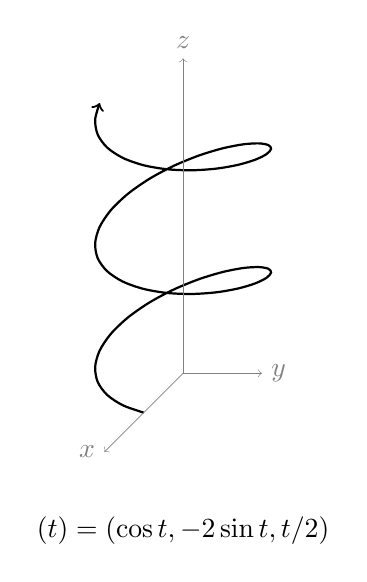
\begin{tikzpicture}
\draw[thick, ->] plot[domain=0:14, smooth, scale=0.5, samples=50]({-2*sin(\x r)-cos(\x r)},{\x/2-cos(\x r)});
\draw (0,-2) node{$\va(t)=(\cos t, -2\sin t, t/2)$};
\draw[help lines, ->] (0,0)--(0,4) node[above]{$z$};
\draw[help lines, ->] (0,0)--(-1,-1) node[left]{$x$};
\draw[help lines, ->] (0,0)--(1,0) node[right]{$y$};
	\end{tikzpicture}
\quad	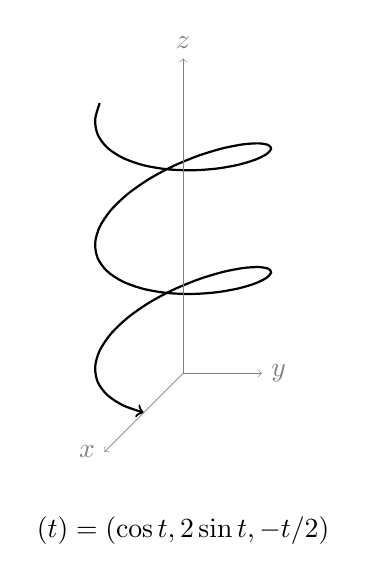
\begin{tikzpicture}
\draw[thick, ->] plot[domain=-14:0, smooth, scale=0.5, samples=50]({-2*sin(-\x r)-cos(\x r)},{-\x/2-cos(\x r)});
\draw (0,-2) node{$\vb(t)=(\cos t, 2\sin t, -t/2)$};
\draw[help lines, ->] (0,0)--(0,4) node[above]{$z$};
\draw[help lines, ->] (0,0)--(-1,-1) node[left]{$x$};
\draw[help lines, ->] (0,0)--(1,0) node[right]{$y$};
\end{tikzpicture}\quad	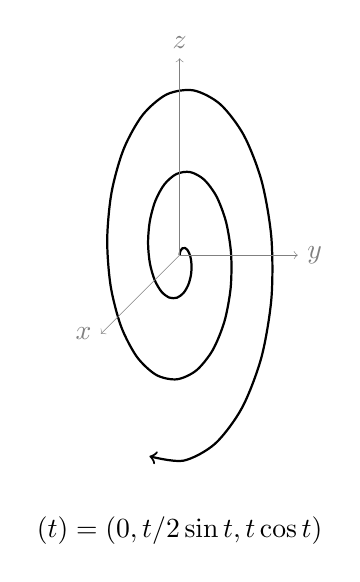
\begin{tikzpicture}
\draw[thick, ->] plot[domain=0:16, smooth, scale=0.5, samples=50]({\x*sin(\x r)/6},{\x/3*cos(\x r)});
\draw (0,-3.5) node{$\vc(t)=(0, t/2\sin t, t\cos t)$};
\draw[help lines, ->] (0,0)--(0,2.5) node[above]{$z$};
\draw[help lines, ->] (0,0)--(-1,-1) node[left]{$x$};
\draw[help lines, ->] (0,0)--(1.5,0) node[right]{$y$};
\end{tikzpicture}
\end{center}
\end{question}
\begin{hint}
Review Example~\eref{CLP317}{eg:helixTwist} %1.4.4
 and remember that positive torsion indicates ``right-handed twisting." You shouldn't actually need to calculate anything.
\end{hint}
\begin{answer}
	$\va(t)$ and $\vb(t)$ have negative torsion,  $\vc(t)$ has zero torsion.
\end{answer}
\begin{solution}
\textbf{Solution 1:}\\
	Curves $\va$ and $\vb$ are the same curve, just parametrized differently (replace $t$ with $-t$ to convince yourself if the picture isn't enough). So, they ought to have the same torsion.
	
	As in  Example~\eref{CLP317}{eg:helixTwist}, we imagine that the curve is the thread on a bolt. Take a look at your right hand. If your thumb is pointing up (corresponding to the $+z$ direction), and you're looking at the tip of your thumb, your fingers curl anticlockwise. Imagine a screw has threads matching the curves $\va$ and $\vb$, and we turn it anticlockwise. The screw would move down --- \emph{not} in the same direction as our thumb. So these curves are not right-handed helices, so they have negative torsion.
	
	The curve $\vc$ sits entirely in a plane (the plane $x=0$) so its torsion is zero everywhere.
	
\textbf{Solution 2:}\\
Here
is the conventional computation for both $\va(t)$ and $\vb(t)$.
(The upper sign is for $\va$ and the lower sign is for $\vb$.)
\begin{align*}
\vr(t)&=\big(\cos t\,,\,\mp 2\sin t \,,\,\pm t/2\big) \\
\vv(t)&=\big(-\sin t\,,\,\mp 2\cos t \,,\,\pm 1/2\big) \\
\va(t)&=\big(-\cos t\,,\,\pm 2\sin t \,,\,0\big) \\
\vv(t)\times\va(t)&=\big(-\sin t\,,\,\mp\cos t/2\,,\,\mp 2\big) \\
\diff{\va}{t}(t)&=\big(\sin t\,,\,\pm 2\cos t\,,\,0\big) \\
\vv(t)\times\va(t)\cdot \diff{\va}{t}(t) &= -1 \\
\tau(t)=\frac{\vv(t)\times\va(t)\cdot \diff{\va}{t}(t)}{|\vv(t)\times\va(t)|^2}
  &=-\frac{1}{\sin^2 t+\frac{1}{4}\cos^2 t+4}
   <0
\end{align*}
\end{solution}
%%%%%%%%%%%%%%%%%%%

%%%%%%%%%%%%%%%%%%%%%%%%%%%
\begin{question}
Consider a curve that is parametrized by arc length $s$.
\begin{enumerate}[(a)]
\item
Show that if the curve has curvature $\ka(s)=0$
for all $s$, then the curve is a straight line.

\item
Show that if the curve has curvature $\ka(s)>0$ and
torsion $\tau(s)=0$ for all $s$, then the curve lies in a plane.

\item
Show that if the curve has curvature $\ka(s)=\ka_0$,
a strictly positive constant, and torsion $\tau(s)=0$
for all $s$, then the curve is a circle.
\end{enumerate}
\end{question}

\begin{hint} 
(a) Show that the tangent vector $\hT(s)$ is a constant.

(b) Guess the plane. To do so, first show that the binormal $\hB(s)$ 
    is a constant. Then show that $(\vr(s)-\vr(0))\cdot\hB $ is a constant.

(c) Guess the circle. To do so, first show that $\vr_c(s)=\vr(s)+\frac{1}{\ka(s)}\hN(s)$ is a constant.

\end{hint}

\begin{answer} 

\end{answer}


\begin{solution}
(a) 
If $\ka(s)\equiv 0$, then 
$\diff{\hT}{s}=\ka(s)\hN(s)\equiv 0$ so that $\hT$ is a constant.
As a result $\diff{\vr}{s}(s)=\hT$ and $\vr(s) =s\hT+\vr(0)$ so that
the curve is the straight line with direction vector $\hT$ that passes
through $\vr(0)$.

(b) If $\tau(s)\equiv 0$, then 
$\diff{\hB}{s}=-\tau(s)\hN(s)\equiv 0$ so that $\hB$ is a constant.
As $\hT(s)\perp\hB$, 
\begin{equation*}
\diff{}{s} (\vr(s)-\vr(0))\cdot\hB =\hT(s)\cdot\hB=0
\end{equation*}
and $ (\vr(s)-\vr(0))\cdot\hB$ must be a constant. The constant
must be zero (set $s=0$), so $ (\vr(s)-\vr(0))\cdot\hB=0$ and $\vr(s)$
always lies in the plane through $\vr(0)$ with normal vector $\hB$.

(c) Parametrize the curve by arc length. Define the ``centre of 
curvature'' at $s$ by
\begin{equation*}
\vr_c(s)=\vr(s)+\frac{1}{\ka(s)}\hN(s)
\end{equation*}
Since $\ka(s)=\ka_0$ is a constant and $\tau(s)\equiv 0$,
\begin{equation*}
\diff{}{s}\vr_c(s)
   =\hT(s)+\frac{1}{\ka_0}\big[\tau(s)\hB-\ka(s)\hT\big]
   =\hT(s)+\frac{1}{\ka_0}\big[0\hB-\ka_0\hT\big]
   =0
\end{equation*}
Thus $\vr_c(s)=\vr_c$ is a constant and 
$\big|\vr(s)-\vr_c\big|=\frac{1}{\ka_0}$ lies on the sphere of radius
$\frac{1}{\ka_0}$ centred on $\vr_c$. Since $\tau(s)\equiv 0$,
the curve also lies on a plane, so it is a circle.
\end{solution}

%%%%%%%%%%%%%%%%%%%%%%%%%%%
\begin{question}[M317 2018A] %2
The surface $z=x^2+y^2$ is sliced by the plane $x=y$.
The resulting curve is oriented from $(0,0,0)$ to $(1,1,2)$.
\begin{enumerate}[(a)]
\item
Sketch the curve from $(0,0,0)$ to $(1,1,2)$.
\item
Sketch $\hat\vT$, $\hat\vN$ and $\hat\vB$ at $\big(\half,\half,\half\big)$.
\item
Find the torsion at $\big(\half,\half,\half\big)$.
\end{enumerate}
\end{question}

\begin{hint} 
It is not necessary to compute anything.
\end{hint}

\begin{answer} 
(a), (b)

\begin{center}
       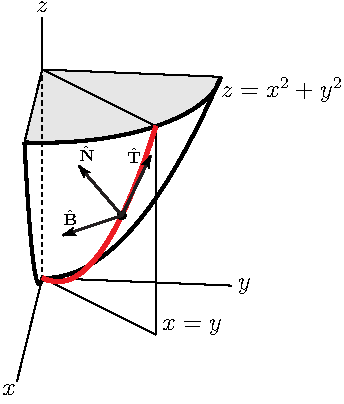
\includegraphics{parabolicBowlB.pdf}
\end{center}

(c) 
The torsion is zero.
\end{answer}

\begin{solution} 
(a), (b): $\hT$ points in the direction of the curve; $\hN$ is perpendicular to it, in the same plane, pointing towards the centre of curvature. Using the right-hand rule in the picture, we see $\hB$ is pointing to the left.

\begin{center}
       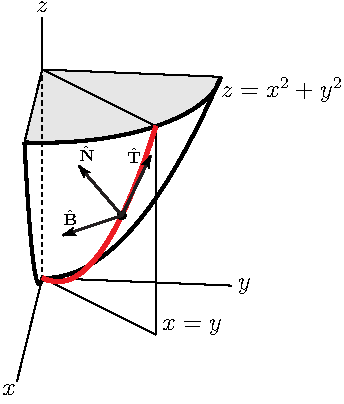
\includegraphics{parabolicBowlB.pdf}
\end{center}

(c) 
The torsion is zero, since the curve lies in a plane (the plane $x=y$).
\end{solution}



%%%%%%%%%%%%%%%%%%
\subsection*{\Procedural}
%%%%%%%%%%%%%%%%%%

%%%%%%%%%%%%%%%%%%%%%%%%%%%
\begin{question}[M317 2006A] %2
Let $C$ be the space curve
\begin{align*}
\vr(t) = \big(e^t - e^{-t}\big)\,\hi + \big(e^t + e^{-t}\big)\,\hj +2t\,\hk
\end{align*}
\begin{enumerate}[(a)]
\item
Find $\vr'$, $\vr''$ and the curvature of $C$.
\item
Find the length of the curve between $\vr(0)$ and $\vr(1)$.
\end{enumerate}
\end{question}

\begin{hint} 
Both parts of this question make use of the quantity $\diff{s}{t}$.
\end{hint}

\begin{answer} 
(a) $\vr'(t)=\big(e^t + e^{-t}\big)\,\hi + \big(e^t - e^{-t}\big)\,\hj +2\,\hk$,
    $\vr''(t)=\big(e^t - e^{-t}\big)\,\hi + \big(e^t + e^{-t}\big)\,\hj$,

\hskip0.75in    $\ka(t) =\frac{1}{2+e^{2t}+e^{-2t}}$

(b) $\sqrt{2}\Big[e-\frac{1}{e}\Big]$
\end{answer}

\begin{solution} (a)
As
\begin{align*}
\vr'(t)&=\big(e^t + e^{-t}\big)\,\hi + \big(e^t - e^{-t}\big)\,\hj +2\,\hk &
\diff{s}{t}(t) &=|\vr'(t)|= \sqrt{4+2e^{2t}+2e^{-2t}}
                =\sqrt{2}\big(e^t+e^{-t}\big)\\
\vr''(t)&=\big(e^t - e^{-t}\big)\,\hi + \big(e^t + e^{-t}\big)\,\hj   &
\vr'(t)\times\vr''(t)&=-2\big(e^t + e^{-t}\big)\,\hi 
          + 2\big(e^t - e^{-t}\big)\,\hj +4\,\hk
\end{align*}
the curvature
\begin{align*}
\ka(t) &= \frac{|\vv(t)\times\va(t)|}{\big(\diff{s}{t}\big)^3}
 =\frac{2\sqrt{4+2e^{2t}+2e^{-2t}}}{[4+2e^{2t}+2e^{-2t}]^{3/2}}
 =\frac{1}{2+e^{2t}+e^{-2t}}
\end{align*}

(b) The length of $C$ between $\vr(0)$ and $\vr(1)$ is
\begin{align*}
\int_0^1 \diff{s}{t}(t) \ \dee{t}
&= \sqrt{2} \int_0^1 (e^t+e^{-t}) \ \dee{t}
=\sqrt{2}\Big[e^t-e^{-t}\Big]_0^1
=\sqrt{2}\Big[e-\frac{1}{e}\Big]
\end{align*}


\end{solution}
%%%%%%%%%%%%%%%%%%%
\begin{question}
	Find the torsion of $\vr(t)=(t,t^2,t^3)$ at the point $(2,4,8)$.
\end{question}
\begin{hint}
	$\tau(t)=\dfrac{(\vv(t) \times \va(t))\cdot\diff{\va}{t}}{|\vv(t) \times \va(t)|^2}$
\end{hint}
\begin{answer}
$\frac{3}{{181}}$
\end{answer}
\begin{solution}
 The point $(2,4,8)$ occurs when $t=2$.
	\begin{align*}
		\vv(t)&=(1,2t,3t^2) & \vv(2)&=(1,4,12)\\
		\va(t)&=(0,2,6t) & \va(2)&=(0,2,12)\\
		\diff{\va}{t}(t)&=(0,0,6) & \diff{\va}{t}(2)&=(0,0,6)\\
		&& \vv(2) \times \va(2)&=(24,-12,2)\\
		&& |\vv(2) \times \va(2)|&=2\sqrt{181}
		\end{align*}
Now, we use a formula for torsion:
\begin{align*}\tau(t)&=\dfrac{(\vv(t) \times \va(t))\cdot\diff{\va}{t}(t)}{|\vv(t) \times \va(t)|^2}\\
\tau(2)&=\frac{(24,-12,2)\cdot(0,0,6)}{(2\sqrt{181})^2}=\frac{3}{{181}}
		\end{align*}
	
\end{solution}

%%%%%%%%%%%%%%%%%%%%%%%%%%%
\begin{question}
Find the unit tangent, unit normal and binormal vectors and
the curvature and torsion of the curve
\begin{equation*}
\vr(t)=t\,\hi + \frac{t^2}{2}\,\hj + \frac{t^3}{3}\,\hk
\end{equation*}
\end{question}

\begin{hint} 
Review \S\eref{CLP317}{sec:CurveCompendium} of the CLP-4 text.
\end{hint}

\begin{answer} 
$\hT(t)=\frac{\hi + t\,\hj + t^2\,\hk}{\sqrt{1+t^2+t^4}}$\qquad
$\hB(t)=\frac{t^2\,\hi-2t\,\hj+\hk}{\sqrt{1+4t^2+t^4}}$\qquad
$\hN(t)=\frac{-(t+2t^3)\,\hi+(1-t^4)\,\hj+(2t+t^3)\hk}
            {\sqrt{1+t^2+t^4}\sqrt{1+4t^2+t^4}}$

$\ka(t)=\frac{\sqrt{1+4t^2+t^4}}{[1+t^2+t^4]^{3/2}}$\qquad
$\tau(t)=\frac{2}{1+4t^2+t^4}$
\end{answer}


\begin{solution}
For the specified curve
\begin{align*}
\vr(t)&=t\,\hi + \frac{t^2}{2}\,\hj + \frac{t^3}{3}\,\hk\\
\vv(t)=\vr'(t)&= \hi + t\,\hj + t^2\,\hk \\
\va(t)=\vr''(t)&= \hj + 2t\,\hk  \\
\vv(t)\times\va(t) 
&=\det\left[\begin{matrix}
                 \hi  & \hj &  \hk \\
                  1   &  t  &  t^2 \\
                  0   &  1  &  2t
       \end{matrix}\right] \\
& = t^2\,\hi-2t\,\hj+\hk\\
\va'(t)&=  2\,\hk  
\end{align*}
From this, we read off
\begin{align*}
\hT(t)&=\frac{\vv(t)}{|\vv(t)|}
        =\frac{\hi + t\,\hj + t^2\,\hk}{\sqrt{1+t^2+t^4}}\\
\ka(t)&=\frac{|\vv(t)\times\va(t)|}{|\vv(t)|^3}
       =\frac{\sqrt{1+4t^2+t^4}}{[1+t^2+t^4]^{3/2}}\\
\hB(t)&=\frac{\vv(t)\times\va(t)}{|\vv(t)\times\va(t)|}
       =\frac{t^2\,\hi-2t\,\hj+\hk}{\sqrt{1+4t^2+t^4}}\\
\hN(t)&=\hB(t)\times\hT(t) \\
       &= \frac{1}{\sqrt{1+t^2+t^4}\sqrt{1+4t^2+t^4}}\det\left[\begin{matrix}
                 \hi  & \hj &  \hk \\
                  t^2 & -2t &  1 \\
                  1   &  t  &  t^2
       \end{matrix}\right] \\ 
       &=\frac{-(t+2t^3)\,\hi+(1-t^4)\,\hj+(2t+t^3)\hk}
            {\sqrt{1+t^2+t^4}\sqrt{1+4t^2+t^4}}\\
\tau(t)&=\frac{\big(\vv(t)\times\va(t)\big)\cdot\va'(t)}{|\vv(t)\times\va(t)|^2}
       =\frac{2}{1+4t^2+t^4}
\end{align*}
\end{solution}

%%%%%%%%%%%%%%%%%%%
\begin{question}
	For some constant $c$, define $\vr(t)=(t^3,t,e^{ct})$. For which value(s) of $c$ is $\tau(5)=0$? For each of those values of $c$, find an equation for the plane containing the osculating circle to the curve at $t=5$.
\end{question}
\begin{hint}
	The vector perpendicular to the plane containing the osculating circle is the binormal vector, $\hB$.
\end{hint}
\begin{answer}
	When $c=0$, the plane is $z=1$.\\
	When $c=1/5$, the plane is $(1/25)x+3y-(30/e)z=-10$.
\end{answer}
\begin{solution}
	First, some preliminaries:
	\begin{align*}
		\vr(t)&=(t^3,t,e^{ct}) & \vr(5)&=(5^3,5,e^{5c})\\
		\vv(t)&=(3t^2,1,ce^{ct}) & \vv(5)&=(3\cdot 5^2,1,ce^{5c})\\
		\va(t)&=(6t,0,c^2e^{ct}) & \va(5)&=(6\cdot 5,0,c^2e^{5c})	\\
		\diff{\va}{t}(t)&=	(6,0,c^3e^{ct})& 	\diff{\va}{t}(5)&=	(6,0,c^3e^{5c})\\
	&&	\vv(5) \times \va(5)&=(c^2e^{5c},15ce^{5c}(2-5c),-30)
		\end{align*}
	Second, we figure out what value of $c$ makes $\tau(5)=0$.
	\begin{align*}
		0&=\tau(5)=\dfrac{(\vv(5) \times \va(5))\cdot\diff{\va}{t}(5)}{|\vv(5) \times \va(5)|^2}\\
		0&=(\vv(5)\times\va(5))\cdot \diff{\va}{t}(5)\\
		&=(c^2e^{5c},15ce^{5c}(2-5c),-30)\cdot (6,0,c^3e^{5c})\\
		&=6c^2e^{5c}(1-5c)\\
		c&=0 \text{ or } c=\frac15
		\end{align*}
	If $c=0$, then $\vr(t)=(t^3,t,1)$, and so the entire curve is contained inside the plane $z=1$. (Its torsion is zero everywhere --- not just at $t=5$.)
	
	Consider the case $c=\frac15$. When $t=5$, our curve (and its osculating circle) passes through the point $\vr(5)=(5^3,5,e)$. The normal vector to the plane of the osculating curve is the binormal vector $\hB(5)=\frac{\vv(5)\times \va(5)}{|\vv(5)\times \va(5)|}$. Since we don't need the normal vector to the plane to be a unit vector, we can take as the normal vector to the plane simply $\vv(5) \times \va(5)$, or $(e/25,3e,-30)$. Then, an equation of the plane containing the osculating circle is $(e/25)x+(3e)y-30z=-10e$. An equivalent equation for this plane is $(1/25)x+3y-(30/e)z=-10$.
\end{solution}
%%%%%%%%%%%%%%%%%%%

\begin{question}[M317 2013D] %1

\begin{enumerate}[(a)]
\item
Consider the parametrized space curve
\begin{equation*}
\vr(t) = \big(t^2 , t, t^3\big)
\end{equation*}
Find an equation for the plane passing through $(1,1,1)$ with normal vector tangent to $\vr$ at that point.
%%%Joel: "normal plane" isn't defined in the text
% normal plane at the point $(1, 1, 1)$. 

\item
Find the curvature of the curve from (a) as a function of the parameter $t$.

\end{enumerate}
\end{question}

\begin{hint} 
(a) The tangent vector of the curve is also a normal vector for the 
specified plane. 

(b) Review \S\eref{CLP317}{sec:CurveCompendium} of the CLP-4 text.
\end{hint}

\begin{answer} 
(a) $2x +y +3z= 6$\qquad
(b) $\ka(t) =\frac{2\sqrt{1+9t^2+9t^4}}{[1+4t^2+9t^4]^{3/2}}$
\end{answer}

\begin{solution} (a) 
Since $\vr'(t) = (2t,1,3t^2)$, we have $\vr'(1)=(2,1,3)$. So the
normal plane must pass through $\vr(1)=(1,1,1)$ and be perpendicular 
to $(2,1,3)$. The equation of the normal plane is then
\begin{equation*}
2(x-1) +(y-1) +3(z-1)=0\qquad
\text{or}\qquad
2x +y +3z= 6
\end{equation*}

\noindent (b)
As
\begin{align*}
\vv(t)=\vr'(t)&=\big(2t,1,3t^2\big) &
\diff{s}{t} &= \sqrt{1+4t^2+9t^4}\\
\va(t)=\vv'(t)&=\big(2,0,6t\big)  &
\vv(t)\times\va(t)&=\big(6t,-6t^2,-2\big)
\end{align*}
the curvature
\begin{align*}
\ka(t) &= \frac{|\vv(t)\times\va(t)|}{\big(\diff{s}{t}\big)^3}
 =\frac{2\sqrt{1+9t^2+9t^4}}{[1+4t^2+9t^4]^{3/2}}
\end{align*}

\end{solution}
%%%%%%%%%%%%%%%%%%%%%%%%%%%
\begin{question}[M317 2005A] %1
	Let $C$ be the osculating circle to the helix 
	$\vr(t) =\big(\cos t\,,\,\sin t\,,\,t\big)$ 
	at the point where $t=\pi/6$. Find:
	\begin{enumerate}[(a)]
		\item
		the radius of curvature of $C$
		\item
		the center of $C$
		\item
		the unit normal to the plane of $C$
	\end{enumerate}
	
	
\end{question}

\begin{hint} 
	Remember $\va(t)=\difftwo{s}{t}(t)\,\hat\vT(t)
	+\ka(t)\big(\diff{s}{t}(t)\big)^2\hat\vN(t)$. Remember also that $\hB$ is orthogonal to $\hT$ and $\hN$, which are in the plane of $C$.
\end{hint}

\begin{answer} 
	(a) $2$\qquad
	(b) $-\frac{\sqrt{3}}{2}\,\hi-\frac{1}{2}\,\hj+\frac{\pi}{6}\,\hk$\qquad
	(c) $\hat\vB =\frac{1}{2\sqrt{2}}\,\hi
	-\frac{\sqrt{3}}{2\sqrt{2}}\,\hj
	+\frac{1}{\sqrt{2}}\,\hk$
\end{answer}

\begin{solution}
	First some preliminaries.
	\begin{align*}
	\vv(t)&=\vr'(t)=-\sin t\,\hi +\cos t\,\hj + \hk  \\
	\va(t)&=\vr''(t)= -\cos t\,\hi -\sin t\,\hj 
	%\\ \diff{\va}{t}(t)&= a\sin t\,\hi -a\cos t\,\hj
	\end{align*}
	
	(a), (b) 
	From $\vv(t)$ we read off
	\begin{align*}
	\diff{s}{t}=|\vv(t)|=\sqrt{2}\qquad
	%\hat\vT(t)= -\frac{a}{\sqrt{a^2+b^2}}\sin t\,\hi
	%           +\frac{a}{\sqrt{a^2+b^2}} \cos t\,\hj
	%           +\frac{b}{\sqrt{a^2+b^2}}\,\hk
	\end{align*}
	From $\va(t)=\difftwo{s}{t}(t)\,\hat\vT(t)
	+\ka(t)\big(\diff{s}{t}(t)\big)^2\hat\vN(t)$, 
	and the fact that $\difftwo{s}{t}=0$, we read off that
	\begin{align*}
	\ka(t)=\Big(\diff{s}{t}(t)\Big)^{-2}|\va|=\frac{1}{2}\qquad
	\hat\vN(t) = \frac{\va}{|\va|}=-\cos t\,\hi-\sin t\,\hj
	\end{align*}
	So radius of curvature is $\frac{1}{\ka}=2$ and the centre of  curvature is
	\begin{align*}
	\left[\vr(t) +\frac{1}{\ka(t)}\hat\vN(t)\right]_{t=\nicefrac{\pi}{6}}
	&=\left[\big(\cos t\,\hi +\sin t\,\hj + t\hk \big)
	+2 \big( -\cos t\,\hi-\sin t\,\hj\big)\right]_{t=\nicefrac{\pi}{6}} \\
	&=\left[-\cos t\,\hi
	-\sin t\,\hj
	+t\,\hk \right]_{t=\nicefrac{\pi}{6}} \\
	&=-\frac{\sqrt{3}}{2}\,\hi-\frac{1}{2}\,\hj+\frac{\pi}{6}\,\hk
	\end{align*}
	
	(c)
	From
	\begin{align*}
	\vv(t)\times\va(t)  &= \det\left[
	\begin{matrix}  \hi   & \hj     & \hk \\
	-\sin t & \cos t &  1 \\
	-\cos t &-\sin t & 0\end{matrix} \right] 
	= \sin t\,\hi -\cos t\,\hj + \hk \\
	|\vv(t)\times\va(t)|^2 &= 2
	\end{align*}
	we read off
	\begin{align*}
	\hat\vB(t) & = \frac{\vv(t)\times\va(t)}{|\vv(t)\times\va(t)|}
	=\frac{1}{\sqrt{2}}\sin t\,\hi
	-\frac{1}{\sqrt{2}} \cos t\,\hj
	+\frac{1}{\sqrt{2}}\,\hk
	\end{align*}
	so that 
	\begin{align*}
	\hat\vB\big(\nicefrac{\pi}{6}\big) 
	=\frac{1}{2\sqrt{2}}\,\hi
	-\frac{\sqrt{3}}{2\sqrt{2}}\,\hj
	+\frac{1}{\sqrt{2}}\,\hk
	\end{align*}
	
\end{solution}
%%%%%%%%%%%%%%%%%%%

\begin{question}[M317 2012D] %1

\begin{enumerate}[(a)]
\item
Consider the parametrized space curve
\begin{equation*}
\vr(t) = (\cos(t), \sin(t), t^2)
\end{equation*}
Find a parametric form for the tangent line at the point corresponding 
to $t = \pi$.
\item
Find the tangential component $a_T(t)$ of acceleration, as a function of $t$, 
for the parametrized space curve $\vr(t)$.% of (a).
\end{enumerate}
\end{question}

\begin{hint} 
By Theorem \eref{CLP317}{thm:curvatureFormulae} of the CLP-4 text,
the tangential component of acceleration is
$
a_T(t) = \difftwo{s}{t}
$
\end{hint}

\begin{answer} 
(a) $\vR(t) = (-1,0,\pi^2)+t(0,-1,2\pi)$\qquad
(b) $a_T(t) =\frac{4t}{\sqrt{1+4t^2}}$
\end{answer}

\begin{solution} (a)
The velocity vector is
\begin{align*}
\vr'(t) = (-\sin(t), \cos(t), 2t)
\end{align*}
So a tangent vector at $t=\pi$ is $\vT= (0,-1,2\pi)$ and a 
parametric form for the tangent line is
\begin{align*}
\vR(t) =\vr(\pi) +t\vT = (-1,0,\pi^2)+t(0,-1,2\pi)
\end{align*}

\noindent (b)
The speed is
\begin{align*}
\diff{s}{t} = |\vr'(t)| = \sqrt{1+4t^2}
\end{align*}
By Theorem \eref{CLP317}{thm:curvatureFormulae} of the CLP-4 text,
the tangential component of acceleration is
\begin{align*}
a_T(t) = \difftwo{s}{t}
       =\diff{\hfill}{t}\sqrt{1+4t^2}
       =\frac{4t}{\sqrt{1+4t^2}}
\end{align*}
\end{solution}

%%%%%%%%%%%%%%%%%%%%%%%%%%%
\begin{question}[M317 2010A]  %2
Suppose, in terms of the time parameter $t$ , a particle moves along the path
$\vr(t) = (\sin t - t \cos t )\,\hi + (\cos t + t \sin t )\,\hj + t^2\,\hk$, 
$1 \le t < \infty$.
\begin{enumerate}[(a)]
\item
Find the speed of the particle at time $t$.
\item
Find the tangential component of acceleration at time $t$.
\item
Find the normal component of acceleration at time $t$.
\item
Find the curvature of the path at time $t$.
\end{enumerate}
\end{question}

\begin{hint} 
Use your answers to previous parts to calculate (d). Tangential and normal components of acceleration are defined just before Example~\eref{CLP317}{eg:curveCircle} in the text.
\end{hint}

\begin{answer} 
(a) $\sqrt{5}\,t$\qquad
(b) $\va_T(t) =  \sin t \,\hi   + \cos t \,\hj   + 2\,\hk$\qquad
(c) $\va_N(t) =  t\cos t \,\hi   - t\sin t \,\hj$ \qquad  

(d) $\ka(t) = \frac{1}{5t}$

\end{answer}

\begin{solution} (a) The velocity vector of the particle at time $t$
is
\begin{align*}
\vr'(t) &= (\cos t - \cos t + t \sin t )\,\hi 
         + (-\sin t + \sin t  +  t \cos t )\,\hj 
         + 2t\,\hk \\
        &=  t \sin t \,\hi 
         +  t \cos t \,\hj 
         + 2t\,\hk
\end{align*}
so its speed at time $1\le t<\infty$ is
\begin{align*}
\diff{s}{t}=|\vr'(t)| & = \sqrt{t^2\sin^2t + t^2\cos^2t +4t^2}
           =\sqrt{5}\, t
\end{align*}


\noindent (b)
The unit tangent at time $t$ is
\begin{equation*}
\hat\vT(T) = \frac{\vr'(t)}{|\vr'(t)|}
           =\frac{1}{\sqrt{5}}\big(  \sin t \,\hi 
                                  + \cos t \,\hj 
                                  + 2\,\hk\big)
\end{equation*}
So the tangential component of acceleration at time $t$ is
\begin{equation*}
\va_T(t) = \difftwo{s}{t}(t)\ \hat\vT(t)
          =  \sin t \,\hi   + \cos t \,\hj   + 2\,\hk
\end{equation*}

\noindent (c)
The (full) acceleration is 
\begin{equation*}
\vr''(t) =\diff{\hfill}{t}\vr'(t)
         = \big(\sin t + t\cos t\big) \,\hi 
         + \big(\cos t - t\sin t\big) \,\hj 
         + 2\,\hk
\end{equation*}
So the normal component of acceleration at time $t$ is
\begin{equation*}
\va_N(t) = \va(t) - \va_T(t)
          =  t\cos t \,\hi   - t\sin t \,\hj  
\end{equation*}

\noindent (d)
Another formula for the normal component of acceleration
is $\ka(t)\big(\diff{s}{t}(t)\big)^2\hat\vN(t)$. So the magnitude
of the normal component of acceleration is $\ka(t)\big(\diff{s}{t}(t)\big)^2$
and, by part (c),
\begin{align*}
\ka(t)\left(\diff{s}{t}(t)\right)^2
=\big|t\cos t \,\hi   - t\sin t \,\hj \big|
=t
\end{align*}
Consequently, by part (a),
\begin{equation*}
\ka(t) = \frac{t}{\left(\diff{s}{t}(t)\right)^2}
       = \frac{1}{5t}
\end{equation*}
\end{solution}

%%%%%%%%%%%%%%%%%%%%%%%%%%%
\begin{question}[M317 2009A] %1
Assume the paraboloid $z = x^2 + y^2$ and the plane $2x + z = 8$ 
intersect in a curve $C$. $C$ is traversed counter-clockwise 
if viewed from the positive $z$-axis.
\begin{enumerate}[(a)]
\item
Parametrize the curve $C$.
\item
Find the unit tangent vector $\hat\vT$, the principal normal vector 
$\hat\vN$, the binormal vector $\hat\vB$ and the curvature $\kappa$ 
all at the point $(2, 0, 4)$.
\end{enumerate}
\end{question}

\begin{hint} 
(a) All points on the curve obey an equation that contains $x$'s and $y$'s,
but no $z$'s. There is a standard way to get a nice parametrization of this equation, that doesn't involve using square roots.

(b) You don't need to compute the constants for all points: only the given point.
\end{hint}

\begin{answer} 
(a) $\vr(\theta) = [-1 + 3\cos\theta]\,\hi
                   +3\sin\theta\,\hj
                   +[10-6\cos\theta]\,\hk$, 
$0\le\theta < 2\pi$

(b) At $(2,0,4)$, $\hat\vT = \hj$, 
                  $\hat\vN = \frac{-\hi+2\hk}{\sqrt{5}}$,
                  $\hat\vB = \frac{2\hi+\hk}{\sqrt{5}}$,
                  $\kappa(0) =\frac{\sqrt{5}}{3}$
\end{answer}

\begin{solution} (a)
If the point $(x,y,z)$ is on the curve, it obeys both 
$z = x^2 + y^2$ and $z = 8-2x$ and hence is also obeys
\begin{equation*}
x^2+y^2 = 8-2x\qquad\text{or}\qquad
   (x+1)^2+y^2 =9
\end{equation*}
So the curve $C$ is also the intersection of
\begin{equation*}
(x+1)^2+y^2 =9\qquad\text{and}\qquad  z = 8-2x
\end{equation*}
$(x+1)^2+y^2 =9$ is the circle of radius $3$ centred on $(-1,0)$ and can
be parametrized by
$x(\theta) = -1 + 3\cos\theta$, $y(\theta) = 3\sin\theta$, $0\le\theta\le 2\pi$.
So $C$ can be parametrized by
\begin{align*}
x(\theta) &= -1 + 3\cos\theta \\
y(\theta) &= 3\sin\theta \\
z(\theta) &= 8-2x(\theta) = 10-6\cos\theta \\
\text{ or }\vr(\theta) &= [-1 + 3\cos\theta]\,\hi
                   +3\sin\theta\,\hj
                   +[10-6\cos\theta]\,\hk
\end{align*}
with $0\le\theta < 2\pi$.

Remark: if we tried to parametrize the equation as $(x,y,z)=(x,\sqrt{8-2x-x^2},8-2x)$, then we would miss the negative $y$-values.

\noindent (b)
Note that $\vr(\theta)$ is $(2,0,4)$ when $\theta=0$.
As
\begin{align*}
\vv(\theta)&=\vr'(\theta) = -3\sin\theta\,\hi
                   +3\cos\theta\,\hj
                   +6\sin\theta\,\hk &
\vv(0)&=3\hj \\
\va(\theta)&=\vv'(\theta) = -3\cos\theta\,\hi
                   -3\sin\theta\,\hj
                   +6\cos\theta\,\hk &
\va(0)&= -3\hi+6\hk
\end{align*}
the unit tangent vector at $(2,0,4)$ is
\begin{align*}
\hat\vT(0) &= \frac{\vv(0)}{|\vv(0)|} =\hj
\end{align*}
and, since $\vv(0)\times\va(0) = 9\hk+18\hi$, the unit binormal vector and 
curvature at $(2,0,4)$ are
\begin{align*}
\hat\vB(0) &= \frac{\vv(0)\times\va(0)}{|\vv(0)\times\va(0)|} 
=\frac{2\hi+\hk}{\sqrt{5}}\qquad
\kappa(0) = \frac{|\vv(0)\times\va(0)|}{|\vv(0)|^3}
=\frac{9\sqrt{5}}{3^3}=\frac{\sqrt{5}}{3}
\end{align*}
and the unit normal vector $\hN$ at $(2,0,4)$
\begin{align*}
\hat\vN(0) = \hat\vB(0) \times \hat\vT(0)
           =\frac{1}{\sqrt{5}} (2\hi+\hk)\times\hj
           =\frac{1}{\sqrt{5}} (2\hk-\hi)
\end{align*}


\end{solution}



%%%%%%%%%%%%%%%%%%%%%%%%%%%
\begin{question}[M317 2008A] %1
Consider the curve $C$ given by
\begin{equation*}
\vr(t) = \frac{1}{3} t^3\,\hi + \frac{1}{\sqrt{2}} t^2\,\hj + t\,\hk,\qquad
-\infty < t < \infty.
\end{equation*}
\begin{enumerate}[(a)]
\item
Find the unit tangent $\hat\vT(t)$ as a function of $t$.
\item
Find the curvature $\kappa(t)$ as a function of $t$.
\item
Determine the principal normal vector $\hat\vN$ at the point 
$\big(\frac{8}{3} , 2\sqrt{2}, 2\big)$.
\end{enumerate}
\end{question}

\begin{hint} 
For part (c), you only need to find $\hN$ at a point, which is easier than finding it for all $t$.
\end{hint}

\begin{answer} 
(a) $\hat\vT(t) = \frac{t^2\,\hi +\sqrt{2}\,t\,\hj +\hk}{t^2+1}$\qquad
(b) $\frac{\sqrt{2}} {{(t^2+1)}^2}$\qquad
(c) $\frac{4\,\hi -3\sqrt{2}\,\hj -4\hk}{\sqrt{50}}$
\end{answer}

\begin{solution} 
We have
\begin{align*}
\vv(t)&=\vr'(t) = t^2\,\hi +\sqrt{2}\,t\,\hj +\hk &
|\vv(t)|&=\sqrt{t^4+2t^2+1}=t^2+1
\\
\va(t)&=\vv'(t) = 2t\,\hi +\sqrt{2}\,\hj
\end{align*}

(a)
The unit tangent vector  is
\begin{align*}
\hat\vT(t) &= \frac{\vv(t)}{|\vv(t)|} 
            = \frac{t^2\,\hi +\sqrt{2}\,t\,\hj +\hk}{t^2+1}
\end{align*}

(b)
Since
\begin{align*}
\vv(t)\times\va(t)&= \det\left[\begin{matrix}
           \hi &  \hj & \hk \\
           t^2   &   \sqrt{2}\,t  & 1 \\
           2t    &   \sqrt{2}     & 0
\end{matrix}\right]
=-\sqrt{2}\,\hi +2t\,\hj-\sqrt{2}\,t^2\,\hk
\end{align*}
The curvature is
\begin{align*}
\kappa(t) = \frac{|\vv(t)\times\va(t)|}{|\vv(t)|^3}
=\frac{\sqrt{2+4t^2+2t^4}} {{(t^2+1)}^3}
=\frac{\sqrt{2}} {{(t^2+1)}^2}
\end{align*}

(c)
Note that $\vr(2)$ is $\big(\frac{8}{3} , 2\sqrt{2}, 2\big)$. 
\begin{description}
\item[\textbf{Solution 1:}]
Since
\begin{align*}
\hat\vT'(t) & = \frac{2t\,\hi +\sqrt{2}\,\hj}{t^2+1}
               -2t\frac{t^2\,\hi +\sqrt{2}\,t\,\hj +\hk}{{(t^2+1)}^2} \\
\hat\vT'(2) & = \frac{4\,\hi +\sqrt{2}\,\hj}{5}
               -4\frac{4\,\hi +2\sqrt{2}\,\hj +\hk}{25} \\
            &=\frac{4\,\hi -3\sqrt{2}\,\hj -4\hk}{25} \\
|\vT'(2)|&=\frac{5\sqrt{2}}{25}
\end{align*}
the principal normal vector $\hN$ at $\big(\frac{8}{3} , 2\sqrt{2}, 2\big)$ is
\begin{align*}
\hat\vN(2) &=\frac{\hat\vT'(2)}{|\hat\vT'(2)|}
           =\frac{4\,\hi -3\sqrt{2}\,\hj -4\hk}{5\sqrt{2}}
\end{align*}

\item[\textbf{Solution 2:}]
Perhaps we'd rather not differentiate $\hT(t)$. 
\begin{align*}
\hB &= \dfrac{\vv(t) \times \va(t)}{|\vv(t) \times \va(t)|} \quad\text{and}\quad \hN=\hB \times \hT
\intertext{ Using our previous work:}
\hB(2)&=\frac{\vv(2) \times \va(2)}{|\vv(2)\times\va(2)|} = \frac{-\sqrt2\hi+4\hj-4\sqrt2\hk}{\sqrt{2+16+32}}=\frac{1}{5}\left(-\hi+{2\sqrt2}\hj-4\hk\right)\\
\hT(2)&=\frac{1}{5}\left(4\hi+2\sqrt2\hj+\hk \right)\\
\hN(2)&=\hB(2)\times\hT(2)=\frac{1}{5}\left(-\hi+{2\sqrt2}\hj-4\hk\right)\times\frac{1}{5}\left(4\hi+2\sqrt2\hj+\hk \right)\\
&=\left(\frac{2\sqrt2}{5}\right)\hi+\left(-\frac35\right)\hj+\left(-\frac{2\sqrt2}{5}\right)\hk
\end{align*}
\end{description}

%\begin{align*}
%\hat\vT(2) &= \frac{4\,\hi +2\sqrt{2}\,\hj +\hk}{5} \\
%\vv(2)\times\va(2)&=-\sqrt{2}\,\hi +4\,\hj-4\sqrt{2}\,\hk
%\end{align*}
%So the unit binormal vector at $\big(\frac{8}{3} , 2\sqrt{2}, 2\big)$ is
%\begin{align*}
%\hat\vB(2) &= \frac{\vv(2)\times\va(2)}{|\vv(2)\times\va(2)|} 
%=\frac{-\sqrt{2}\,\hi +4\,\hj-4\sqrt{2}\,\hk}{\sqrt{50}}
%\end{align*}
%and the principal normal vector at $\big(\frac{8}{3} , 2\sqrt{2}, 2\big)$ is
%\begin{align*}
%\hat\vN(2) = \hat\vB(2) \times \hat\vT(2)
%\end{align*}


\end{solution}

%%%%%%%%%%%%%%%%%%%%%%%%%%%
\begin{question}[M317 2007A] %1
Suppose the curve $C$ is the intersection of the cylinder $x^2 +y^2 = 1$ 
with the plane $x+y+z = 1$.
\begin{enumerate}[(a)]
\item
Find a parameterization of $C$.
\item
Determine the curvature of $C$.
\item
Find the points at which the curvature is maximum and determine the value
of the curvature at these points.
\end{enumerate}
\end{question}

\begin{hint} 
First parametrize $x^2+y^2=1$ in the standard way. You don't need calculus for part (c).
\end{hint}

\begin{answer} 
(a) One possible parametrization is 
$\vr(\theta) = \cos\theta\,\hi +\sin\theta\,\hj + (1-\cos\theta-\sin\theta)\,\hk$ with $0\le\theta\le 2\pi$.

(b) $\ka(\theta)=\frac{\sqrt{3}}{[2-\sin(2\theta)]^{3/2}}$

(c) $\text{maximum curvature }=\sqrt{3}$
    at $\frac{\hi}{\sqrt{2}}+\frac{\hj}{\sqrt{2}}+(1-\sqrt{2})\,\hk$
    and $-\frac{\hi}{\sqrt{2}}-\frac{\hj}{\sqrt{2}}+(1 + \sqrt{2})\,\hk$\\
 $\text{\hskip0.25in minimum curvature }= \frac{1}{3}$\quad\ 
         at $-\frac{\hi}{\sqrt{2}}+\frac{\hj}{\sqrt{2}}+\hk$
         and $\frac{\hi}{\sqrt{2}}-\frac{\hj}{\sqrt{2}}+\hk$

\end{answer}

\begin{solution} (a)
The curve $x^2+y^2=1$ is a circle of radius $1$.
So we can parametrize it by $x(\theta)=\cos\theta$, 
$y(\theta)=\sin\theta$, $0\le\theta<2\pi$. The $z$-coordinate of any point on
the intersection is determined by $z=1-x-y$. So we can use
\begin{equation*}
\vr(\theta) = \cos\theta\,\hi +\sin\theta\,\hj + (1-\cos\theta-\sin\theta)\,\hk
\qquad 0\le\theta<2\pi
\end{equation*}

(b) 
As
\begin{align*}
\vv(\theta)=\vr'(\theta)&=\big(-\sin\theta,\cos\theta,\sin\theta-\cos\theta\big) \\
\va(\theta)=\vv'(\theta)&=\big(-\cos\theta,-\sin\theta,\cos\theta+\sin\theta\big)
\end{align*}
we have
\begin{align*}
\diff{s}{\theta} &= |\vr'(\theta)|
=\sqrt{\sin^2\theta+\cos^2\theta+(\sin\theta-\cos\theta)^2}\\
&=\sqrt{2-2\sin\theta\cos\theta} \\
&=\sqrt{2-\sin(2\theta)} \\
\vv(\theta)\times\va(\theta)&=\big(1,1,1\big)
\end{align*}
and the curvature
\begin{align*}
\ka(\theta) &= \frac{|\vv(\theta)\times\va(\theta)|}{\big(\diff{s}{\theta}\big)^3}
 =\frac{\sqrt{3}}{[2-\sin(2\theta)]^{3/2}}
\end{align*}

(c) The curvature is 
\begin{itemize}\itemsep1pt \parskip0pt \parsep0pt %\itemindent-15pt
\item[$\circ$] 
a maximum (minimum) when $2-\sin(2\theta)$
is a minimum (maximum), 
\item[$\circ$]
which is the case when $\sin(2\theta)=1$
($\sin(2\theta)=-1$), 
\item[$\circ$]
which in turn is the case when $\theta=\frac{\pi}{4},\frac{5\pi}{4}$
($\theta=\frac{3\pi}{4},\frac{7\pi}{4}$). 
\end{itemize}
So
\begin{align*}
\text{maximum curvature }&= \frac{\sqrt{3}}{[2-1]^{3/2}}=\sqrt{3} &&
\text{at }\qquad\frac{\hi}{\sqrt{2}}+\frac{\hj}{\sqrt{2}}+(1-\sqrt{2})\,\hk \\
& &&
\text{and }\quad-\frac{\hi}{\sqrt{2}}-\frac{\hj}{\sqrt{2}}+(1+\sqrt{2})\,\hk \\
\text{minimum curvature }&= \frac{\sqrt{3}}{[2-(-1)]^{3/2}}=\frac{1}{3} &&
\text{at }\qquad-\frac{\hi}{\sqrt{2}}+\frac{\hj}{\sqrt{2}}+\hk \\
& &&
\text{and }\qquad\frac{\hi}{\sqrt{2}}-\frac{\hj}{\sqrt{2}}+\hk 
\end{align*}

\end{solution}


%%%%%%%%%%%%%%%%%%%%%%%%%%%%
\begin{question}[M317 2006D] %6
Let
\begin{align*}
\vr(t) = t^2\,\hi + 2t\,\hj + \ln t\,\hk
\end{align*}
Compute the unit tangent and unit normal vectors $\hat\vT(t)$ and $\hat\vN(t)$. Compute the curvature $\kappa(t)$. Simplify whenever possible!
\end{question}

\begin{hint} 
Review \S\eref{CLP317}{sec:CurveCompendium} of the CLP-4 text.
\end{hint}

\begin{answer} 
$\hat\vT(t) =\frac{2t^2\,\hi + 2t\,\hj + \hk}{2t^2+1}$\qquad
$\hat\vN(t) =\frac{2t\,\hi - (2t^2-1)\,\hj -2t\, \hk}{2t^2+1}$\qquad
$\ka(t) = \frac{2t}{{(2t^2+1)}^2}$
\end{answer}

\begin{solution}
For $\vr(t)$ to be well-defined, we need $t>0$ (because of the $\ln t$.)
\begin{align*}
\vv(t)=\vr'(t)&=2t\,\hi + 2\,\hj + \frac{1}{t}\,\hk &
\diff{s}{t} &= \sqrt{4t^2+4+\nicefrac{1}{t^2}}
              =2t+\frac{1}{t} 
\end{align*}
The unit tangent vector is
\begin{align*}
\hat\vT(t) = \frac{\vr'(t)}{|\vr'(t)|}
           =\frac{2t\,\hi + 2\,\hj + \frac{1}{t}\,\hk}{2t+\frac{1}{t}}
           =\frac{2t^2\,\hi + 2t\,\hj + \hk}{2t^2+1}
\end{align*}
so, from  \S\eref{CLP317}{sec:CurveCompendium} of the CLP-4 text,
\begin{align*}
\diff{s}{t}(t)\, \ka(t)\,\hat\vN(t) &= \hat\vT'(t)
                 =\frac{4t\,\hi + 2\,\hj }{2t^2+1}
                  -4t\frac{2t^2\,\hi + 2t\,\hj + \hk}{{(2t^2+1)}^2}
                 =\frac{4t\,\hi + (-4t^2+2)\,\hj -4t\, \hk}{{(2t^2+1)}^2} \\
&=2\frac{2t\,\hi - (2t^2-1)\,\hj -2t\, \hk}{{(2t^2+1)}^2}
\end{align*}
Since the length of $2t\,\hi - (2t^2-1)\,\hj -2t\, \hk$ is
\begin{align*}
\sqrt{4t^2 + (2t^2-1)^2+4t^2}
&=\sqrt{8t^2 + 4t^4 -4 t^2 + 1}
=\sqrt{ 4t^4 +4 t^2 + 1} \\
&=\sqrt{(2t^2+1)^2} 
=2t^2+1
\end{align*}
we have
\begin{align*}
\hat\vN(t) =\frac{2t\,\hi - (2t^2-1)\,\hj -2t\, \hk}{2t^2+1}
\end{align*}
and
\begin{align*}
\ka(t) = \frac{|\hat\vT'(t)|}{\diff{s}{t}(t)}
=\frac{\frac{2}{2t^2+1}}{2t+\frac{1}{t}}
=\frac{2t}{{(2t^2+1)}^2}
\end{align*}
\end{solution}


%%%%%%%%%%%%%%%%%%%%%%%%%%%%%%%%%%%%%%%%%%%%%%

\begin{question}[M317 2015A]  %1 c,d,e

\begin{enumerate}[(a)]
\item
Find the length of the curve  $\vr(t)=\big(1,\frac{t^2}{2},\frac{t^3}{3}\big)$
for $0\le t\le 1$.

\item
Find the principal unit normal vector $\hN$ to $\vr(t) = \cos(t)\,\hi + \sin(t)\,\hj 
+ t\,\hk$ at $t =\pi/4$.

\item
Find the curvature of $\vr(t) = \cos(t)\,\hi + \sin(t)\,\hj + t\,\hk$ 
at $t = \pi/4$.

\end{enumerate}
\end{question}

\begin{hint} 
	Since $0 \le t \le 1$, you can simplify $|t|=t$.
\end{hint}

\begin{answer} 
(a) $\frac{1}{3}\big[2^{3/2}-1\big]$\qquad
(b) $\frac{-\hi - \hj}{\sqrt{2}}$\qquad
(c) $\frac{1}{2}$
\end{answer}

\begin{solution} (a)
Since
\begin{align*}
\vr(t)&= \hi +\frac{t^2}{2}\,\hj + \frac{t^3}{3}\,\hk \\
\vr'(t)&= t\,\hj + t^2\,\hk \\
\diff{s}{t}(t)=|\vr'(t)|&=\sqrt{t^2+t^4}=t\sqrt{1+t^2}
\end{align*}
the length of the curve is
\begin{align*}
\int_0^1 \diff{s}{t}(t)\,\dee{t}
=\int_0^1 t\sqrt{1+t^2}\,\dee{t}
=\frac{1}{3}{\big[1+t^2\big]}^{3/2}\Big|_0^1
=\frac{1}{3}\big[2^{3/2}-1\big]
\end{align*}

(b) For the specified curve
\begin{align*}
\vr(t) &= \cos(t)\,\hi + \sin(t)\,\hj  + t\,\hk \\
\vr'(t) &= -\sin(t)\,\hi + \cos(t)\,\hj  + 1\,\hk \\
\hat\vT(t) &=\frac{-\sin(t)\,\hi + \cos(t)\,\hj  + 1\,\hk}{\sqrt{2}} \\
\hat\vT'(t) &=\frac{-\cos(t)\,\hi - \sin(t)\,\hj}{\sqrt{2}} \\
\hat\vT'\big(\nicefrac{\pi}{4}\big) &=\frac{-\hi - \hj}{2} \\
\hat\vN\big(\nicefrac{\pi}{4}\big) 
&=\frac{\hat\vT'\big(\nicefrac{\pi}{4}\big)}
       {|\hat\vT'\big(\nicefrac{\pi}{4}\big)|}
=\frac{-\hi - \hj}{\sqrt{2}} \\
\end{align*}

(c) Recalling, from \S\eref{CLP317}{sec:CurveCompendium} in the CLP-4 text, 
that
\begin{align*}
\hat\vT'(t) 
=\ka(t) \,\diff{s}{t}(t)\,\hat\vN(t)
\end{align*}
we have, by part (d),
\begin{align*}
\ka\big(\nicefrac{\pi}{4}\big)
&=\frac{|\hat\vT'\big(\nicefrac{\pi}{4}\big)|}
       {|\vr'\big(\nicefrac{\pi}{4}\big)|}
=\frac{1/\sqrt{2}}{\sqrt{2}}
=\frac{1}{2}
\end{align*}
\end{solution}

%%%%%%%%%%%%%%%%%%%%%%%%%%%%%%%%%%%%%%%%%%%%
\begin{question}[M317 2015A]  %7
A particle moves along a curve with position vector given by
\begin{equation*}
\vr(t) = \big(t + 2\,,\, 1 - t\,,\, t^2 /2\big)
\end{equation*}
for $-\infty < t < \infty$.

\begin{enumerate}[(a)]
\item
Find the velocity as a function of $t$.

\item
Find the speed as a function of $t$.

\item
Find the acceleration as a function of $t$.

\item
Find the curvature as a function of $t$.

\item
Recall that the decomposition of the acceleration into tangential and
normal components is given by the formula
\begin{equation*}
\vr''(t) = \difftwo{s}{t} \hat\vT(t) 
 + \kappa(t)\Big(\diff{s}{t}\Big)^2\hat\vN(t)
\end{equation*}
Use this formula and your answers to the previous parts of this 
question to find $\hat\vN(t)$, the principal unit normal vector,
as a function of $t$.

\item
Find an equation for the osculating plane (the plane which best fits the curve) at the point corresponding to $t = 0$.

\item
Find the centre of the osculating circle at the point corresponding 
to $t = 0$.

\end{enumerate}
\end{question}

\begin{hint} 
For part (f), remember that you can write the equation of a plane easily once you know a point it passes through, and a vector normal to it. The plane should touch the curve when $t=0$, and the plane should contain $\hT$ and $\hN$.
\end{hint}

\begin{answer} 
(a) $\vv(t) = \big(1\,,\, -1\,,\, t\big)$\qquad
(b) $\diff{s}{t}(t)=\sqrt{2+t^2}$\qquad
(c) $\va(t) =\big(0\,,\, 0\,,\, 1\big)$\

(d) $\ka(t) = \frac{\sqrt{2}}{{[2+t^2]}^{3/2}}$\qquad
(e) $\hat\vN(t) = \frac{(-t\,,\, t\,,\, 2)}{\sqrt{2(2+t^2)}}$\qquad
(f) $x+y = 3$\qquad
(g) $(2,1,2)$
\end{answer}

\begin{solution}  (a), (b), (c)
We have
\begin{align*}
\vr(t) &= \big(t + 2\,,\, 1 - t\,,\, t^2 /2\big) \\
\vv(t) =\vr'(t)&= \big(1\,,\, -1\,,\, t\big) \\
\diff{s}{t}(t)=|\vv(t)|&=\sqrt{2+t^2} \\
\va(t) = \vv'(t)&=\big(0\,,\, 0\,,\, 1\big) 
\end{align*}

(d) By \S\eref{CLP317}{sec:CurveCompendium} of the CLP-4 text,
the curvature
\begin{align*}
\ka(t) & = \frac{|\vv(t)\times\va(t)|}{(\diff{s}{t}(t))^3}
= \frac{|(-1,-1,0)|}{{[2+t^2]}^{3/2}}
= \frac{\sqrt{2}}{{[2+t^2]}^{3/2}}
\end{align*}

(e) Since $\diff{s}{t}(t)=\sqrt{2+t^2}$, we have 
$\difftwo{s}{t}(t)=\frac{t}{\sqrt{2+t^2}}$ and
\begin{align*}
\big(0\,,\, 0\,,\, 1\big) 
=\va(t) 
&= \difftwo{s}{t} \hat\vT(t) 
 + \kappa(t)\Big(\diff{s}{t}\Big)^2\hat\vN(t) \\
&=\frac{t}{\sqrt{2+t^2}}\,\frac{(1\,,\, -1\,,\, t)}{\sqrt{2+t^2}} 
  + \frac{\sqrt{2}}{{[2+t^2]}^{3/2}}\big(\sqrt{2+t^2}\big)^2\hat\vN(t)
\end{align*}
or
\begin{align*}
\frac{\sqrt{2}}{\sqrt{2+t^2}}\hat\vN(t)
=\big(0\,,\, 0\,,\, 1\big)  - \frac{(t\,,\, -t\,,\, t^2)}{2+t^2} 
=\frac{(-t\,,\, t\,,\, 2)}{2+t^2} 
\end{align*}
which implies
\begin{align*}
\hat\vN(t) = \frac{(-t\,,\, t\,,\, 2)}{\sqrt{2(2+t^2)}}
\end{align*}

(f) At $t=0$
\begin{align*}
\vr(0) &= (2,1,0) \\
\hat\vT(0)&= \frac{(1,-1,0)}{\sqrt{2}} \\
\hat\vN(0)&= (0,0,1) \\
\hat\vB(0)&= \hat\vT(0)\times\hat\vN(0)
           = \frac{1}{\sqrt{2}}(1,-1,0)\times (0,0,1)
           = \frac{1}{\sqrt{2}}(-1 ,-1, 0)
\end{align*}
The osculating plane is the plane through $\vr(0)$ which is perpendicular
to $\hat\vB(0)$, which is
\begin{equation*}
\frac{1}{\sqrt{2}}(-1 ,-1, 0)\cdot\big\{(x,y,z) - (2,1,0)\big\}=0
\qquad\text{or}\qquad
x+y = 3
\end{equation*}

(g) The osculating circle has centre
\begin{equation*}
\vr(0)+\frac{1}{\ka(0)}\hat\vN(0)
=(2,1,0) +\frac{1}{1/2} (0,0,1)
=(2,1,2)
\end{equation*}
\end{solution}


%%%%%%%%%%%%%%%%%%%%%%%%%%%%%%%
\begin{question}[M317 2012J] %5
Consider the curve $C$ given by
\begin{equation*}
\vr(t) =\frac{t^3}{3}\,\hi + \frac{t^2}{\sqrt{2}}\,\hj + t\,\hk \qquad
-\infty < t < \infty
\end{equation*}
\begin{enumerate}[(a)]
\item
Find the unit tangent $\hat\vT(t)$ as a function of $t$.
\item
Find the curvature $\kappa(t)$ as a function of $t$.
\item
Evaluate $\kappa(t)$ at $t = 0$.
\item
Determine the principal normal vector $\hat\vN(t)$ at $t = 0$.
\item
Compute the binormal vector $\hat\vB(t)$ at $t = 0$.
\end{enumerate}
\end{question}

\begin{hint} 
It might be easier to find $\hB$ before you find $\hN$, then use the formula $\hN(t)=\hB(t)\times\hT(t)$.
\end{hint}

\begin{answer} 
(a) $\hat\vT(t)=\frac{t^2\,\hi + \sqrt{2} t\,\hj + \hk}{t^2+1}$\qquad
(b) $\ka(t) =\frac{\sqrt{2}}{{(t^2+1)}^2}$\qquad
(c) $\ka(0) = \sqrt{2}$\qquad
(d) $\hat\vN(0) = \hj$\qquad

(e) $\hat\vB(0) = -\hi$
\end{answer}

\begin{solution} 
First some preliminary computations.
\begin{align*}
\vr(t) &=\frac{t^3}{3}\,\hi + \frac{t^2}{\sqrt{2}}\,\hj + t\,\hk \\
\vr'(t) &=t^2\,\hi + \sqrt{2} t\,\hj + \hk &
|\vr'(t)|&= \sqrt{t^4+2t^2+1} =t^2+1\\
\vr''(t) &=2t\,\hi + \sqrt{2}\,\hj \displaybreak[0]\\
\vr'(t)\times\vr''(t)&= \det\left[\begin{matrix}\hi&\hj&\hk\\[0.03in] 
     t^2 & \sqrt{2} t & 1\\
     2t  & \sqrt{2} & 0\end{matrix}\right]
=-\sqrt{2}\,\hi +2t\,\hj -\sqrt{2} t^2\,\hk \hidewidth
\end{align*}

(a) The unit tangent vector is
\begin{align*}
\hat\vT(t) = \frac{\vr'(t)}{|\vr'(t)|}
      =\frac{t^2\,\hi + \sqrt{2} t\,\hj + \hk}{t^2+1}
\end{align*}

(b) The curvature is (see \S\eref{CLP317}{sec:CurveCompendium} of the CLP-4 text)
\begin{align*}
\ka(t)  &= \frac{|\vr'(t)\times\vr''(t)|}{|\vr'(t)|^3}
=\frac{|-\sqrt{2}\,\hi +2t\,\hj -\sqrt{2} t^2\,\hk|}{{(t^2+1)}^3}
=\frac{\sqrt{2+4t^2+2t^4}}{{(t^2+1)}^3} \\
&=\frac{\sqrt{2}}{{(t^2+1)}^2}
\end{align*}

(c) At $t=0$
\begin{equation*}
\ka(0) = \sqrt{2}
\end{equation*}

For ease of computation, we'll find $\hB$ first, then use it to find $\hN$.

(e) At $t=0$, the binormal vector is (see \S\eref{CLP317}{sec:CurveCompendium} of the CLP-4 text)
\begin{align*}
\hat\vB(0) = \frac{\vr'(0)\times\vr''(0)}{|\vr'(0)\times\vr''(0)|}
          = \frac{-\sqrt{2}\,\hi}{\sqrt{2}}
          =-\hi
\end{align*}

(d) At $t=0$, the principal normal vector is (see \S\eref{CLP317}{sec:CurveCompendium} of the CLP-4 text)
\begin{align*}
\hat\vN(0) = \hat\vB(0)\times\hat\vT(0) 
           =-\hi \times\hk
           =\hj
\end{align*}
\end{solution}


%%%%%%%%%%%%%%%%%%%%%%%%%%%%%%%
\begin{question}[M317 2016D] %1
A curve in $\bbbr^3$ is given by $\vr(t) = (t^2\,,\, t\,,\, t^3)$.
\begin{enumerate}[(a)]
\item
Find the parametric equations of the tangent line to the curve at the point 
$(1, -1, -1)$.
\item
Find an equation for the osculating plane of the curve at the point 
$(1, 1, 1)$.
\end{enumerate}
\end{question}

\begin{hint} 
The osculating plane at $\vr(t_0)$ is the plane through
$\vr(t_0)$ with normal $\hat\vB(t_0)$. Also, notice the points for parts (a) and (b) are not the same.
\end{hint}

\begin{answer} 
(a) $x=1-2t$, 
$y=-1+t$,
$z=-1+3t$\qquad
(b) $3x-3y-z = -1$
\end{answer}

\begin{solution} 
The curve has
\begin{align*}
\vr(t) &= (t^2\,,\, t\,,\, t^3) \\
\vv(t)= \vr'(t) &= (2t\,,\, 1\,,\, 3t^2) \\
\va(t)= \vr''(t) &= (2\,,\, 0\,,\, 6t) 
\end{align*}

(a) In particular, a (non unit) tangent vector at $\vr(-1) = (1, -1, -1)$
is $\vr'(-1) = (-2, 1,3)$. So the tangent line to the curve at
$(1, -1, -1)$ is
\begin{align*}
(x,y,z) - (1, -1, -1) = t (-2, 1, 3)
\end{align*}
or
\begin{align*}
x&=1-2t \\
y&=-1+t \\
z&=-1+3t
\end{align*}

(b) At $\vr(1)= (1,1,1)$,
\begin{align*}
\vv(1)= \vr'(1) &= (2, 1, 3) \\
\va(1)= \vr''(1) &= (2, 0, 6) \\
\vv(1)\times\va(1) &= (6,-6,-2)
\end{align*}
So the unit binormal vector is
\begin{equation*}
\hat\vB(1) = \frac{\vv(1)\times \va(1)}{|\vv(1)\times \va(1)|}
           =\frac{(3,-3,-1)}{|(3,-3,-1)|}
           =\frac{1}{\sqrt{19}} (3,-3,-1)
\end{equation*}
An equation for the osculating plane is
\begin{equation*}
(3,-3,-1)\cdot(x-1\,,\,y-1\,,\,z-1) = 0\qquad\text{or}\qquad
3x-3y-z = -1
\end{equation*}
\end{solution}

%%%%%%%%%%%%%%%%%%%%%%%%%%%%%%%
\begin{question}[M317 2016D] %2
A curve in $\bbbr^3$ is given by
\begin{equation*}
\vr(t) = (\sin t - t \cos t)\,\hi + (\cos t + t \sin t)\,\hj + t^2\,\hk,
\qquad
0 \le t < \infty
\end{equation*}
\begin{enumerate}[(a)]
\item
Find the length of the curve $\vr(t)$ from $\vr(0) = (0, 1, 0)$ to 
$\vr(\pi) = (\pi, -1, \pi^2)$.
\item
Find the curvature of the curve at time $t > 0$.
\end{enumerate}
\end{question}

\begin{hint} 
Since $t>0$, we can simplify $\sqrt{t^2}=|t|=t$.
\end{hint}

\begin{answer} 
(a) $\frac{\sqrt{5}\,\pi^2}{2}$\qquad
(b) $\ka(t) = \frac{1}{5t}$
\end{answer}

\begin{solution} (a) For this curve
\begin{align*}
\vr'(t) &= t\sin t\,\hi + t\cos t\,\hj +2t\,\hk \\
\diff{s}{t}(t)=|\vr'(t)| &= \sqrt{5} \,t
\end{align*}
so the length of the curve from $t=0$ to $t=\pi$ is
\begin{align*}
\int_0^\pi \diff{s}{t}(t)\, \dee{t}
=\sqrt{5} \int_0^\pi t\, \dee{t}
=\frac{\sqrt{5}\,\pi^2}{2}
\end{align*}

(b) The unit tangent vector is
\begin{equation*}
\hat T(t) = \frac{\vr'(t)}{|\vr'(t)|} 
     = \frac{1}{\sqrt{5}}\big(\sin t\,\hi + \cos t\,\hj +2\,\hk\big)
\end{equation*}
so that
\begin{align*}
\ka(t)\,\diff{s}{t}(t)\,\hat\vN(t) = \diff{\hat\vT}{t}(t)
=\frac{1}{\sqrt{5}}\big(\cos t\,\hi - \sin t\,\hj \big)
\end{align*}
which implies that
\begin{align*}
\ka(t)\overbrace{\sqrt{5}\, t}^{\diff{s}{t}(t)}
=\frac{1}{\sqrt{5}}\big|\big(\cos t\,\hi - \sin t\,\hj \big)\big|
=\frac{1}{\sqrt{5}}
\implies  \ka(t) = \frac{1}{5t}
\end{align*}
\end{solution}




%%%%%%%%%%%%%%%%%%%%%%%%%%%
\begin{question}[M317 2004A] %1
At time $t=0$, NASA launches a rocket which follows a
trajectory so that its position at any time $t$ is
\begin{equation*}
x=\frac{4\sqrt{2}}{3}t^{3/2},\ y=\frac{4\sqrt{2}}{3}t^{3/2},\ z=t(2-t)
\end{equation*}
\begin{enumerate}[(a)]
\item
Assuming that the flight ends when $z=0$, find out how far
the rocket travels.
\item 
Find the unit tangent and unit normal to the trajectory
at its highest point.
\item 
Also, compute the curvature of the trajectory at its highest point.
\end{enumerate}

\end{question}

\begin{hint} 
	In this context, ``distance travelled" means ``arclength."
\end{hint}

\begin{answer} 
(a) $8$\qquad
(b) $\hat\vT(1)=\frac{1}{\sqrt{2}}(1,1,0)$,
    $\hat\vN(1) = (0,0,-1)$\qquad
(c) $\ka(1) =\frac{1}{8}$
\end{answer}

\begin{solution} 
(a) 
For the specified curve
\begin{align*}
\vr(t)&=\left(\frac{4\sqrt{2}}{3}t^{3/2},\frac{4\sqrt{2}}{3}t^{3/2},
            t(2-t)\right)\\
\vv(t)&=\big(2\sqrt{2}t^{1/2},2\sqrt{2}t^{1/2},2-2t\big)\\
|\vv|&=\sqrt{8t+8t+4-8t+4t^2}=\sqrt{4(1+2t+t^2)}= 2(1+t)
\end{align*}
The rocket is at $z=0$ when $t=0$ and when $t=2$.
So the distance travelled is 
\begin{align*}
\int_0^2|\vv(t)|\,dt=\int_0^2 2(1+t)\,dt = 2\left[t+\frac{t^2}{2}\right]_0^2
=8
\end{align*}

(b) The rocket is at its maximum height when $\diff{z}{t}=2-2t=0$.
That is, when $t=1$. Its velocity then is $(2\sqrt{2},2\sqrt{2},0)$. A
unit vector in this direction is $\hat\vT(1)=\frac{1}{\sqrt{2}}(1,1,0)$.
That is the unit tangent vector. 

At general $t$, the unit tangent is
\begin{equation*}
\hat\vT(t) = \frac{\vv(t)}{|\vv(t)|}
           = \frac{\big(\sqrt{2}t^{1/2},\sqrt{2}t^{1/2},1-t\big)}{1+t} 
\end{equation*}
So
\begin{align*}
\hat\vT'(t)  &= \frac{\big(\sqrt{2}t^{-1/2}/2,\sqrt{2}t^{-1/2}/2,-1\big)}{1+t}
              -\frac{\big(\sqrt{2}t^{1/2},\sqrt{2}t^{1/2},1-t\big)}{(1+t)^2} \\
\hat\vT'(1)  &= \frac{\big(\sqrt{2}/2,\sqrt{2}/2,-1\big)}{2}
              -\frac{\big(\sqrt{2},\sqrt{2},0\big)}{4} \\
              &= \big(0,0, -\nicefrac{1}{2}\big)
\end{align*}
So the principal unit normal vector is
\begin{equation*}
\hat\vN(1) = \frac{\hat\vT'(1)}{|\hat\vT'(1)|} = (0,0,-1)
\end{equation*}

(c) As
\begin{align*}
\diff{\hat\vT}{t}(1)  = \big(0,0, -\nicefrac{1}{2}\big)\qquad
\diff{s}{t}(1) = |\vv(1)| = 4
\end{align*}
the curvature
\begin{align*}
\ka(1) &= \frac{|\hat\vT'(1)|}{|\vv(1)|}
=\frac{1}{8}
\end{align*}

%(c) As
%\begin{align*}
%\vv(t)=\vr'(t)&=\big(2\sqrt{2}t^{1/2},2\sqrt{2}t^{1/2},2-2t\big) &
%\vv(1)&=2\sqrt{2}\big(1,1,0\big)\\
%\va(t)=\vv'(t)&=\big(\sqrt{2}t^{-1/2},\sqrt{2}t^{-1/2},-2\big) &
%\va(1)&=\sqrt{2}\big(1,1,-\sqrt{2}\big)\\
%\vv(1)\times\va(1)&=4\big(-\sqrt{2},\sqrt{2},0\big) &
%|\vv(1)|&=4
%\end{align*}
%the curvature
%\begin{align*}
%\ka(1) &= \frac{|\vv(1)\times\va(1)|}{|\vv(1)|^3}
% =\frac{8}{4^3}
%=\frac{1}{8}
%\end{align*}
\end{solution}

%%%%%%%%%%%%%%%%%%%%%%%%%%%
\begin{question}[M317 2001A] %1
Consider a particle travelling in space along the 
path parametrized by  
\begin{equation*}
x=\cos^3t,\ y=\sin ^3t,\ z=2\sin^2 t
\end{equation*}
\begin{enumerate}[(a)]
\item
Calculate the arc length of this path for $0\le t\le \pi/2$.

\item
Find the vectors $\hat\vT$, $\hat\vN$, $\hat\vB$ for 
the particle at $t=\pi/6$.
\end{enumerate}
\end{question}

\begin{hint} 
Use $\hT$ and $\hN$ to compute $\hB$.
\end{hint}

\begin{answer} 
(a) $\frac{5}{2}$

(b) $\hat\vT\big(\nicefrac{\pi}{6}\big)
           =\frac{1}{5}\Big(-\frac{3}{2},\frac{3\sqrt{3}}{2}, 4\Big)$,   
    $\hat\vN\big(\nicefrac{\pi}{6}\big) 
               =\frac{1}{2}\big(\sqrt{3},1,0\big)$, 
    $\hat\vB(\nicefrac{\pi}{6}\big)
          =\frac{1}{5}\big(-2,2\sqrt{3},-3)$ 
\end{answer}


\begin{solution}
(a)  For the specified curve
\begin{align*}
\vr(t)&=\big(\cos^3t,\sin^3t,2\sin^2t\big)\\
\vv(t)&=\big(-3\cos^2t\sin t,3\sin^2t\cos t,4\sin t\cos t\big)
=\sin t\cos t (-3\cos t,3\sin t, 4)\\
|\vv(t)|&=\sin t\cos t\sqrt{9\cos^2t+9\sin^2t+16}=5\sin t\cos t
\end{align*}
So the distance travelled is 
\begin{equation*}
\int_0^{\pi/2}|\vv(t)|\,\dee{t}=\int_0^{\pi/2} 5\sin t\cos t\,\dee{t} = \frac{5}{2}\sin^2t\Big|_0^{\pi/2}
=\frac{5}{2}
\end{equation*}

(b) Since
\begin{align*}
\vv(t)&=\sin t\cos t (-3\cos t,3\sin t, 4) &
|\vv(t)|&=5\sin t\cos t
\end{align*}
we have
\begin{align*}
\hat\vT(t) &= \frac{\vv(t)}{|\vv(t)|} 
           =\frac{1}{5}(-3\cos t,3\sin t, 4) &
\hat\vT\big(\nicefrac{\pi}{6}\big)
           &=\frac{1}{5}\Big(-\frac{3}{2},\frac{3\sqrt{3}}{2}, 4\Big) \\
\hat\vT'(t) &=\frac{1}{5}(3\sin t,3\cos t, 0) &
\hat\vT'\big(\nicefrac{\pi}{6}\big)
           &=\frac{1}{5}\Big(\frac{3\sqrt{3}}{2}, \frac{3}{2}, 0\Big)
            = \frac{3}{10} \Big(\sqrt{3}, 1, 0\Big)\\
\hat\vN\big(\nicefrac{\pi}{6}\big) &= \frac{\hat\vT'\big(\nicefrac{\pi}{6}\big)}
                                     {|\hat\vT'\big(\nicefrac{\pi}{6}\big)|}
                  =\frac{1}{2}\big(\sqrt{3},1,0\big) &
\hat\vB(\nicefrac{\pi}{6}\big)
&= \hat\vT\big(\nicefrac{\pi}{6}\big)\times
             \hat\vN\big(\nicefrac{\pi}{6}\big) \\
& & &=\frac{1}{10}\big(-4,4\sqrt{3},-6) \\
& & &=\frac{1}{5}\big(-2,2\sqrt{3},-3) 
\end{align*}
\end{solution}


%%%%%%%%%%%%%%%%%%%%%%%%%%%
\begin{question}
Suppose that  the curve $C$ is the intersection of the cylinder $x^2 +y^2 = 1$ 
with the surface  $z =x^2 - y^2$.
\begin{enumerate}[(a)]
\item 
Find a parameterization of $C$.

\item
Determine the curvature of $C$ at the point
            $\big(1/\sqrt{2}\,,1/\sqrt{2}\,,\,0\big)$.

\item
Find the osculating plane to $C$ at the point $\big(1/\sqrt{2}\,,1/\sqrt{2}\,,\,0\big)$.
In general, the osculating plane to a curve $\vr(t)$ at the point
$\vr(t_0)$ is the plane which fits the curve best at $\vr(t_0)$.
It passes through $\vr(t_0)$ and has normal vector $\hat\vB(t_0)$.

\item 
Find the radius and the centre of the osculating circle to $C$ at the 
point $\big(1/\sqrt{2}\,,1/\sqrt{2}\,,\,0\big)$.
\end{enumerate}
\end{question}

\begin{hint} 
(a) First find a parametrization $\big(x(\theta),y(\theta)\big)$
for  $x^2+y^2=1$.
\end{hint}

\begin{answer} 
(a) $\vr(\theta) =\cos\theta\,\hi +\sin\theta\,\hj + \cos(2\theta)\,\hk$
                        \qquad $0\le\theta<2\pi$\qquad 
(b) $\frac{1}{5}$

(c) $z =\sqrt{2}\,x-\sqrt{2}\,y$

(d) radius $1/\ka(\pi/4)=5$ and centre
            $\big(-2\sqrt{2}\,,\,-2\sqrt{2}\,,\,0\big)$
\end{answer}


\begin{solution}
(a)
The curve $x^2+y^2=1$ is a circle of radius $1$.
So we can parametrize it by $x(\theta)=\cos\theta$, 
$y(\theta)=\sin\theta$, $0\le\theta<2\pi$. The $z$-coordinate of any point on
the intersection is determined by $z=x^2-y^2$. So we can use the
parametrization
\begin{align*}
\vr(\theta) &= \cos\theta\,\hi +\sin\theta\,\hj + [\cos^2\theta-\sin^2\theta]\,\hk\\
            &=\cos\theta\,\hi +\sin\theta\,\hj + \cos(2\theta)\,\hk
                        \qquad 0\le\theta<2\pi 
\end{align*}

(b) 
Note that $\vr(\theta) = \big(1/\sqrt{2}\,,1/\sqrt{2}\,,\,0\big)$
when $\theta=\frac{\pi}{4}$.
For general $\theta$, the velocity and acceleration are
\begin{align*}
\vv(\theta)=\vr'(\theta)&=-\sin\theta\,\hi + \cos\theta\,\hj  -2\sin(2\theta)\,\hk \\
\va(\theta)=\vv'(\theta)&=-\cos\theta\,\hi -\sin\theta\,\hj  -4\cos(2\theta)\,\hk
\end{align*}
In particular,
\begin{align*}
\vv(\pi/4)&=-\frac{1}{\sqrt{2}}\,\hi + \frac{1}{\sqrt{2}}\,\hj  -2\,\hk \\
\va(\pi/4)&=-\frac{1}{\sqrt{2}}\,\hi -\frac{1}{\sqrt{2}}\,\hj   \\
\diff{s}{\theta}(\pi/4) &= |\vv(\pi/4)|=\sqrt{5}\\
\vv(\pi/4)\times\va(\pi/4)&=-\sqrt{2}\,\hi +\sqrt{2}\,\hj + \hk\\
|\vv(\pi/4)\times\va(\pi/4)|&=\sqrt{5}
\end{align*}
So the curvature
\begin{equation*}
\ka(\pi/4) = \frac{|\vv(\pi/4)\times\va(\pi/4)|}{|\vv(\pi/4)|^3}
 =\frac{1}{5}
\end{equation*}

(c) The binormal to $C$ at $\big(1/\sqrt{2}\,,1/\sqrt{2}\,,\,0\big)$ is
\begin{align*}
\hat\vB(\pi/4) =\frac{\vv(\pi/4)\times\va(\pi/4)}{|\vv(\pi/4)\times\va(\pi/4)|}
                     =\frac{-\sqrt{2}\,\hi +\sqrt{2}\,\hj + \hk}{\sqrt{5}}
\end{align*}
So the osculating plane to $C$ at $\big(1/\sqrt{2}\,,1/\sqrt{2}\,,\,0\big)$ is
\begin{align*}
&\big(-\sqrt{2}\,,\,\sqrt{2}\,,\,1\big)\cdot\big(x-1/\sqrt{2}\,,\,y-1/\sqrt{2}\,,\,z-0\big) = 0
\qquad{\rm or}\\
& z =\sqrt{2}\,x-\sqrt{2}\,y
\end{align*}

(d) From the computations in parts (b) and (c), we have
\begin{align*}
\hT(\pi/4)&=\frac{\vv(\pi/4)}{|\vv(\pi/4)|}
        =\frac{-1/\sqrt{2}\,\hi + 1/\sqrt{2}\,\hj -2\,\hk}{\sqrt{5}}\\
\hB(\pi/4)&=\frac{\vv(\pi/4)\times\va(\pi/4)}{|\vv(\pi/4)\times\va(\pi/4)|}
       =\frac{-\sqrt{2}\,\hi +\sqrt{2}\,\hj + \hk}{\sqrt{5}}\\
\hN(\pi/4)&=\hB(\pi/4)\times\hT(\pi/4)
       =\frac{-\hi-\hj}{\sqrt{2}}
\end{align*}
So the osculating circle has radius $1/\ka(\pi/4)=5$ and centre
\begin{align*}
\vr_c(\pi/4)&=\vr(\pi/4)+\frac{\hN(\pi/4)}{\ka(\pi/4)}
                 =\big(1/\sqrt{2}\,,1/\sqrt{2}\,,\,0\big)
                   -5\big(1/\sqrt{2}\,,1/\sqrt{2}\,,\,0\big) \\
            &=\big(-2\sqrt{2}\,,\,-2\sqrt{2}\,,\,0\big)
\end{align*}
\end{solution}




%%%%%%%%%%%%%%%%%%
\subsection*{\Application}
%%%%%%%%%%%%%%%%%%


%%%%%%%%%%%%%%%%%%%%%%%%%%%
\begin{question}[M317 2008D] %3
Under the influence of a force field $\vF$, a particle of mass 2 kg is 
moving with constant speed 3 m/s along the path given as the 
intersection of the plane $z = x$ and the parabolic cylinder $z = y^2$, 
in the direction of increasing $y$. Find $\vF$  at the point
$(1, 1, 1)$. (Length is measured in m along the three coordinate axes.)
\end{question}

\begin{hint} 
You need to find the acceleration at $(1,1,1)$. Think about 
what strategies are available for computing the acceleration.
\end{hint}

\begin{answer} 
$\frac{4}{9}(\hi-4\,\hj+\hk)$
\end{answer}

\begin{solution} We'll solve this problem twice, using two different
strategies. (The second strategy will be much more efficient than 
the first one.)
Both strategies use that $\vF=m\va$. Since we are told that 
$m=2$, we just have to find the acceleration $\va$ at $(1,1,1)$.

\noindent \emph{Strategy 1:}\ \ \ In the first strategy, we'll find 
the position $\vr(t)$, as a function of time $t$ and then differentiate
twice to get the acceleration $\va(t)$. 

\begin{itemize}\itemsep1pt \parskip0pt \parsep0pt %\itemindent-15pt
\item[$\circ$] First we'll find any old parametrization.
We are told that, on the path, $z=x$ and $z=y^2$. So let's use $y$ as the
parameter. Then $x=z=y^2$. So the parametrization is
$\vR(y)=y^2\,\hi+ y\,\hj +y^2\,\hk$. (We'll save the notation ``$\vr(t)$''
for the parametrization with respect to time.)

\item[$\circ$] Next we'll reparametrize to get the time $t$ as the parameter.
Since 
\begin{align*}
\diff{\vR}{y} &= 2y\,\hi+\hj + 2y\,\hk \\
\implies \diff{s}{y} &=\big|2y\,\hi+\hj + 2y\,\hk\big|
                      =\sqrt{1+8y^2}
\end{align*}
We are told that the speed $\diff{s}{t}=3$ for all $t$.
So, choosing our zero point for time to coincide with our zero point 
for $s$, we have $s=3t$, or $t=s/3$ so that
\begin{equation*}
\diff{t}{y} =\frac{1}{3}\sqrt{1+8y^2}
\end{equation*}
We could now integrate to get $t$ as a function of $y$. But that
looks quite messy. Fortunately we only need the acceleration at one point,
namely $(1,1,1)$. We'll now see that that saves quite a bit of work.
Pretend that we have integrated to get $t$ as a function of $y$ and call the
answer $t(y)$. Call the inverse function, which gives $y$ as a function of $t$, $y(t)$. 

\item[$\circ$] We now have $\vr(t) = \vR\big(y(t)\big)$. 
So, by the chain rule,
\begin{align*}
\vr'(t) &= \vR'\big(y(t)\big)\ y'(t) \\
\vr''(t) &= \vR'\big(y(t)\big)\ y''(t) + \vR''\big(y(t)\big)\ y'(t)^2
\end{align*}
We're only interest in the time, call it $t_0$, at which $y(t_0)=1$.
The acceleration at time $t_0$ is
\begin{align*}
\vr''(t_0) 
&= \vR'\big(y(t_0)\big)\ y''(t_0) + \vR''\big(y(t_0)\big)\ y'(t_0)^2 \\
& = \vR'(1)\ y''(t_0) + \vR''(1)\ y'(t_0)^2 \\
& = \big[2\,\hi+\hj + 2\,\hk\big]\ y''(t_0) 
         + \big[2\,\hi+ 2\,\hk\big]\ y'(t_0)^2 
\end{align*}
so we just have to find $y'(t_0)$ and $y''(t_0)$.

\item[$\circ$] We know that $\diff{t}{y} =\frac{1}{3}\sqrt{1+8y^2}$.
So by the inverse function theorem
\begin{align*}
\diff{y}{t}(t) 
   &=\frac{3}{\sqrt{1+8y(t)^2}} \\
\difftwo{y}{t}(t) 
   &=-\frac{1}{2}\,\frac{3\big(16y(t)y'(t)\big)}{{[1+8y(t)^2]}^{3/2}} \\
\end{align*}
In particular 
\begin{align*}
y'(t_0) 
   &=\frac{3}{\sqrt{1+8y(t_0)^2}}
    =\frac{3}{\sqrt{1+8}}
    =1 \\
y''(t_0) 
   &=-\frac{24\,y(t_0)y'(t_0)}{{[1+8y(t_0)^2]}^{3/2}}
    = - \frac{24\times 1\times 1}{{(1+8)}^{3/2}}
    = - \frac{8}{9}
\end{align*}

\item[$\circ$] \emph{Finally}, the force is 
\begin{align*}
2\vr''(t_0) &= 2\big[2\,\hi+\hj + 2\,\hk\big]\ y''(t_0) 
         + 2\big[2\,\hi+ 2\,\hk\big]\ y'(t_0)^2  \\
&= -\frac{16}{9}\big[2\,\hi+\hj + 2\,\hk\big] +2\big[2\,\hi+ 2\,\hk\big] \\
&= \frac{4}{9}\,\hi -\frac{16}{9}\,\hj + \frac{4}{9}\,\hk
\end{align*}
\end{itemize}

\noindent \emph{Strategy 2:}\ \ \ The second strategy will be based on
(see \S\eref{CLP317}{sec:CurveCompendium} in the CLP-4 text)
\begin{equation*}
\va=\difftwo{s}{t}\,\hat\vT +\ka\Big(\diff{s}{t}\Big)^2\hat\vN
\end{equation*}
In this problem, we are told that $\diff{s}{t}=3$ for all $t$,
so that $\difftwo{s}{t}=0$ and
\begin{equation*}
\va=9\ka\hat\vN
\end{equation*}
So we just have to find the curvature, $\ka$, and unit normal, $\hat\vN$,
at $(1,1,1)$. We have already found one parametrization of the path
in strategy 1, namely
\begin{equation*}
\vR(y)=y^2\,\hi+ y\,\hj +y^2\,\hk
\end{equation*}
Note that $\vR(1) = (1,1,1)$. Since
\begin{align*}
\vR'(y)&=2y\,\hi+ \hj +2y\,\hk \\
\hat\vT(y)&=\frac{\vR'(y)}{|\vR'(y)|}
           =\frac{2y\,\hi+ \hj +2y\,\hk}{\sqrt{1+8y^2}} 
\\
\hat\vT'(y)&= \frac{2\,\hi +2\,\hk}{\sqrt{1+8y^2}}
                 -\frac{16y}{2}\ \frac{2y\,\hi+ \hj +2y\,\hk}{[1+8y^2]^{3/2}}
\\
\hat\vT'(1)&= \frac{2\,\hi +2\,\hk}{3}
                 -8\frac{2\,\hi+ \hj +2\,\hk}{27}
            =\frac{2\,\hi-8\,\hj +2\,\hk}{27}
\end{align*}
we have (again see \S\eref{CLP317}{sec:CurveCompendium} in the CLP-4 text)
\begin{align*}
\ka(1) &=\frac{|\hat\vT'(1)|}{|\vR'(1)|}
%        =\frac{\sqrt{2^2+8^2+2^2}}{27\times\sqrt{1+8\times 1^2}}
%        =\frac{\sqrt{72}}{3^4}
%        =\frac{2\sqrt{2}}{27}
\\
\hat\vN(1) &=\frac{\hat\vT'(1)}{|\hat\vT'(1)|} \\
\vF&=m\va = 2\times 9\ka(1)\hat\vN(1)
=18\frac{\hat\vT'(1)}{|\vR'(1)|}
=18\frac{2\,\hi-8\,\hj +2\,\hk}{27\sqrt{1+8\times 1^2}} \\
&=\frac{4}{9}(\hi-4\,\hj+\hk)
\end{align*}

\end{solution}

%%%%%%%%%%%%%%%%%%%%%%%%%%%%%%%%%%%
\begin{question}[M317 2016A]  %6
Consider the curve $C$ in 3 dimensions given by
\begin{equation*}
\vr(t) = 2t\hi + t^2\hj + \sqrt{3} t^2\hk
\end{equation*}
for $t \in\bbbr$.

\begin{enumerate}[(a)]
\item
Compute the unit tangent vector $\vT(t)$.

\item
Compute the unit normal vector $\vN(t)$.


\item 
Show that the binormal vector $\vB$ to this curve does not depend on 
$t$ and is one of the following vectors:
\begin{equation*}
\text{\textcircled{1}}\ \left[\begin{matrix}
                  1/2 \\
                  -\sqrt{3}/2 \\
                 0
                \end{matrix}\right]\qquad
\text{\textcircled{2}}\ \left[\begin{matrix}
                  0  \\
                  \sqrt{3}/2 \\
                  1/2
                \end{matrix}\right]\qquad
\text{\textcircled{3}}\ \left[\begin{matrix}
                  0 \\
                  -\sqrt{3}/2 \\
                  1/2
                \end{matrix}\right]\qquad
\text{\textcircled{4}}\ \left[\begin{matrix}
                  0\\
                  -1/2 \\
                  \sqrt{3}/2 
                \end{matrix}\right]\qquad
\end{equation*}
This implies that $C$ is a plane curve.

\item
According to your choice of vector \textcircled{1}, \textcircled{2},
\textcircled{3} or \textcircled{4}, give the equation of the plane
containing $C$.

\item
Compute the curvature $\kappa(t)$ of the curve.


\item
Are there point(s) where the curvature is maximal? If yes, give the 
coordinates of the point(s). If no, justify your answer.

\item
Are there point(s) where the curvature is minimal? If yes, give 
the coordinates of the point(s). If no, justify your answer.

\item
Let 
\begin{equation*}
\vu := 2\,\hi,\quad 
\vv := \hj + \sqrt{3}\,\hk\quad
\vw := -\sqrt{3}\,\hj + \hk
\end{equation*}
   \begin{enumerate}[(i)] 
      \item
      Express $\hi$, $\hj$, $\hk$ in terms of $\vu$, $\vv$, $\vw$.
      \item
      Using (i), write $\vr(t)$ in the form
      \begin{equation*}
                a(t)\vu + b(t)\vv + c(t)\vw
      \end{equation*}
       where $a(t)$, $b(t)$ and $c(t)$ are functions you have to determine. 
       You should find that one of these functions is zero.
     \item
      Draw the curve given by $\big(a(t), b(t)\big)$ in the $xy$-plane.
     \item 
     Is the drawing consistent with parts (f) and (g)? Explain.
     \end{enumerate}
\end{enumerate}
\end{question}

\begin{hint} 
For part (a), $\vT(t)$ will be a vector of the form 
$\vT(t) = \frac{(1,at,bt)}{\sqrt{1+4t^2}}$
where $a$ and $b$ are nonzero constant real numbers.

For part (b), $\vN(t)$ will be a vector of the form 
$\vN(t) = \frac{(-4t,\alpha, \beta)}{2\sqrt{1+4t^2}}$
where $\alpha$ and $\beta$ are nonzero constant real numbers.

For part (e),  $\kappa(t)$ will be a function of the form 
 $\kappa(t) = \frac{\gamma}{{(1+4t^2)}^{3/2}}$, where $\gamma$ is 
a positive constant real number.

\end{hint}

\begin{answer} 
(a) $\hat\vT(t)=\frac{\hi + t\hj + \sqrt{3} t\hk }{\sqrt{1+4t^2}}$\quad
(b) $\hat\vN(t)=\frac{-4t\,\hi + \hj + \sqrt{3} \hk }{2\sqrt{1+4t^2}}$\quad
(c) \textcircled{3}  \quad
(d) $-\sqrt{3} y + z=0$ \quad

(e) $\ka(t)={(1+4t^2)}^{-3/2}$\quad

(f) The curvature $\ka(t)$ achieves its maximum value at $\vr(0)=(0,0,0)$.\quad

(g) The curvature never achieves a minimum.

(h) $\hi=\frac{\vu}{2}$, 
    $\hj=\frac{\vv-\sqrt{3}\,\vw}{4}$,
    $\hk=\frac{\sqrt{3}\,\vv+\vw}{4}$,
    $\vr(t) = t\,\vu + t^2 \,\vv$

\begin{center}
       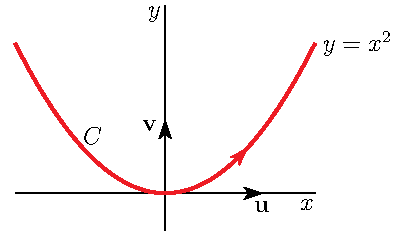
\includegraphics{OE16A_6h.pdf}
\end{center}

The curve $\big(a(t),b(t)\big)=(t,t^2)$ is the curve $y=x^2$.
It is ``curviest'' at the origin, which is consistent with part (f).
It becomes flatter and flatter as $|t|$ increases, but never achieves
``perfect flatness'', which is consistent with (g).


\end{answer}

\begin{solution} (a)
As
\begin{align*}
\vr(t) = 2t\hi + t^2\hj + \sqrt{3} t^2\hk \\
\vr'(t) = 2\hi + 2t\hj + 2\sqrt{3} t\hk 
%\vr'(t) =  2\hj + 2\sqrt{3}\hk
\end{align*}
the unit tangent vector is
\begin{align*}
\hat\vT(t) &=\frac{\hi + t\hj + \sqrt{3} t\hk }{|\hi + t\hj + \sqrt{3} t\hk |}
=\frac{\hi + t\hj + \sqrt{3} t\hk }{\sqrt{1+4t^2}}
\end{align*}


\noindent (b)
Since
\begin{align*}
\diff{\hat\vT}{t}(t)
&=\frac{ \hj + \sqrt{3} \hk }{\sqrt{1+4t^2}}
-4t\frac{\hi + t\hj + \sqrt{3} t\hk }{{(1+4t^2)}^{3/2}}
=\frac{-4t\hi + \hj + \sqrt{3} \hk }{{(1+4t^2)}^{3/2}}
\end{align*}
the unit normal is
\begin{align*}
\hat\vN(t) &=\frac{-4t\hi + \hj + \sqrt{3} \hk }
           {|-4t\hi + \hj + \sqrt{3} \hk|}
=\frac{-4t\,\hi + \hj + \sqrt{3} \hk }{2\sqrt{1+4t^2}}
\end{align*}

\noindent (c) 
The unit binormal is
\begin{align*}
\hat\vB(t) &= \hat\vT(t)\times \hat\vN(t) \\
&=\frac{1}{2(1+4t^2)}\det\left[\begin{matrix}
           \hi &  \hj & \hk \\
           1   &   t  &\sqrt{3} t \\
           -4t &   1  &\sqrt{3}
\end{matrix}\right] \\
&=\frac{-\sqrt{3}(1+4t^2)\hj  + (1+4t^2)\hk}{2(1+4t^2)} \\
&=-\frac{\sqrt{3}}{2}\hj +\frac{1}{2}\hk
\end{align*}
which is \textcircled{3}.

\noindent (d)
The plane contains the point $\vr(0)=\vZero$ and is perpendicular to the
vector $-\frac{\sqrt{3}}{2}\hj +\frac{1}{2}\hk$ and so is
\begin{equation*}
-\sqrt{3} y + z=0
\end{equation*}

\noindent (e)
The curvature is
\begin{align*}
\ka(t) &= \Big|\diff{\hat\vT}{t}(t)\Big|/\Big|\diff{s}{t}\Big|
=\frac{|-4t\hi + \hj + \sqrt{3} \hk| }{{(1+4t^2)}^{3/2}}
  \frac{1}{|2\hi + 2t\hj + 2\sqrt{3} t\hk |} \\
&=\frac{\sqrt{4+16t^2}}{{(1+4t^2)}^{3/2}}  \frac{1}{2\sqrt{1+4t^2}}
=\frac{1}{{(1+4t^2)}^{3/2}}
\end{align*}

\noindent (f), (g)
The denominator ${(1+4t^2)}^{3/2}$ of $\ka(t)$ is a minimum at $t=0$ and grows
without bound as $|t|$ increases. So the denominator never achieves
a maximum. Consquently, the curvature $\ka(t)$ achieves its
maximum value when $t=0$ and so at $\vr(0)=(0,0,0)$. The curvature
never achieves a minimum.

\noindent (h)
Since 
$\sqrt{3}\,\vv+\vw=4\,\hk$ and $\vv-\sqrt{3}\,\vw=4\,\hj$,
\begin{equation*}
\hi=\frac{\vu}{2}\qquad
\hj=\frac{\vv-\sqrt{3}\,\vw}{4}\qquad
\hk=\frac{\sqrt{3}\,\vv+\vw}{4}
\end{equation*}
Since $\vu=2\,\hi$ and $\vv=\hj+\sqrt{3}\,\hk$,
\begin{align*}
\vr(t) = t\,\vu + t^2 \,\vv
= a(t)\vu + b(t)\vv + c(t)\vw
\qquad\text{ with }a(t)=t,\ b(t)=t^2,\ c(t)=0
\end{align*}
The curve $\big(a(t),b(t)\big)=(t,t^2)$ is the curve $y=x^2$.
It is ``curviest'' at the origin, which is consistent with part (f).
It becomes flatter and flatter as $|t|$ increases, but never achieves
``perfect flatness'', which is consistent with (g).

\begin{center}
       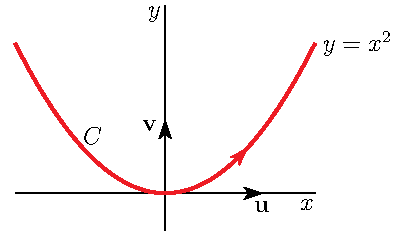
\includegraphics{OE16A_6h.pdf}
\end{center}

\intremark{
Aside from an overall factor of $\frac{1}{2}$, the change of coordinates
is orthogonal.
}


\end{solution}



%%%%%%%%%%%%%%%%%%%%%%%%%%%%%%%
\begin{question}[M317 2017D] %5
Recall that if $\hat\vT$ is the unit tangent vector to an oriented curve 
with arclength parameter $s$, then the curvature $\ka$ and the principle
normal vector $\hat\vN$ are defined by the equation
\begin{equation*}
\diff{\hat\vT}{s} = \ka\,\hat\vN
\end{equation*}
Moreover, the torsion $\tau$ and the binormal vector $\hat\vB$ are defined by
the equations
\begin{equation*}
\hat\vB = \hat\vT\times\hat\vN,\qquad
\diff{\hat\vB}{s} = -\tau\,\hat\vN
\end{equation*} 
Show that
\begin{equation*}
\diff{\hat\vN}{s} = -\ka\,\hat\vT + \tau\,\hat\vB
\end{equation*}
\end{question}

\begin{hint} 
Differentiate $\hat\vN =\hat\vB\times\hat\vT$ with respect to $s$. 

The vectors $\hN, \hB,$ and $\hT$ form a right-handed triple. Sketch them (the same way you might sketch the $x$, $y$, and $z$ axes) to figure out the signs of their cross products.
\end{hint}

\begin{answer} 
See the solution.
\end{answer}

\begin{solution} 
The three unit vectors $\hat\vT$, $\hat\vN$ and $\hat\vB$ are 
mutually perpendicular and form a right handed triple.
\begin{center}
     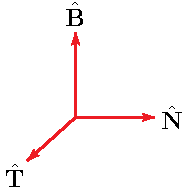
\includegraphics{OE17D_5.pdf}
\end{center}
So
\begin{equation*}
\hat\vN = \hat\vB\times\hat\vT \qquad
\hat\vN\times\hat\vT = -\hat\vB \qquad
\hat\vB\times\hat\vN = -\hat\vT
\end{equation*}
and
\begin{align*}
\diff{\hat\vN}{s} & = \diff{\hat\vB}{s}\times\hat\vT
                     +\hat\vB\times \diff{\hat\vT}{s}
= -\tau\,\hat\vN\times\hat\vT
                     +\hat\vB\times\big(\ka\hat\vN\big)
= \tau\,\hat\vB - \ka\hat\vT
\end{align*}
\end{solution}


%%%%%%%%%%%%%%%%%%%%%%%%%%%
\begin{question}[M317 2000D] %1
 A skier descends the hill $z =\sqrt{4-x^2-y^2}$ along a trail with 
parameterization
$$
x=\sin(2\theta),\qquad y=1-\cos(2\theta),\qquad z=2\cos\theta,\qquad
 0\le\theta\le\frac{\pi}{2}
$$
   Let $P$ denote the point on the trail where $x = 1$.
\begin{enumerate}[(a)]
\item
   Find the vectors $\hat\vT, \hat\vN, \hat\vB$ and 
   the curvature $\ka$ of the ski trail at the point $P$.
                                                         
\item
The skier's acceleration at $P$ is $\va = (-2, 3, -2\sqrt{2})$.
           Find, at $P$,
\begin{enumerate}[(i)]
\item
the rate of change of the skier's speed and
\item
the skier's velocity (a vector).
\end{enumerate}
\end{enumerate}

\end{question}

\begin{hint} 
In part (b), note that $\va$ is the second derivative with respect
       to time (not $\theta$). Exploit $\va = \diff{v}{t}\hat\vT + v^2\kappa\hat\vN$ to  find what you're asked for.
\end{hint}

\begin{answer} 
(a) $\hat\vT = \frac{1}{\sqrt6}\big(0,2,-\sqrt2\big)$,
    $\hat\vN = -\frac{1}{\sqrt{39}}\big(6,1,\sqrt2\big)$,
    $\hat\vB = \frac{1}{\sqrt{13}}\big(-1,2,2\sqrt2\big)$,
    $\kappa = \frac{\sqrt{13}}{3\sqrt3} = \frac{\sqrt{39}}{9}$

(b) (i) $\diff{v}{t}=\frac{5\sqrt2}{\sqrt3}$\qquad (ii) $\vv = (0,\sqrt2,-1)$.
\end{answer}

\begin{solution} (a)
Parametrizing the curve by $\theta$ gives
\begin{align*}
\vr(\theta) &= \big(\sin(2\theta),1-\cos(2\theta),2\cos\theta\big),
\\
\vv =\vr'(\theta)&= \big(2\cos(2\theta),2\sin(2\theta),-2\sin\theta\big),
\\
\va = \vr''(\theta)&=\big(-4\sin(2\theta),4\cos(2\theta),-2\cos\theta\big).
\end{align*}
At the point $P$, we have $\theta=\pi/4$, giving instantaneous
values
$$
\vr = (1,1,\sqrt2),
\quad
\vv = \big(0,2,-\sqrt2\big),
\quad
v = |\vv| = \sqrt6,
\quad
\va = \big(-4,0,-\sqrt2\big).
$$
Hence $\hat\vT = \frac{\vv}{|\vv|} 
   = \frac{1}{\sqrt6}\big(0,2,-\sqrt2\big)$.


Now $\hat\vB = \frac{\vv\times\va}{|\vv\times\va|}
%= \frac{1}{\sqrt{26}}\big(-2\sqrt2,4\sqrt2,8\big)
= \frac{1}{\sqrt{26}}\big(-\sqrt2,2\sqrt2,4\big)
= \frac{1}{\sqrt{13}}\big(-1,2,2\sqrt2\big)$,
since
$$
\vv\times\va
= \left|\begin{matrix}\hi & \hj & \hk \\
0 & 2 & -\sqrt2 \\
-4 & 0 & -\sqrt2 \end{matrix}\right|
= \big(-2\sqrt2,4\sqrt2,8\big),
\qquad
|\vv\times\va| = \sqrt{104} = 2\sqrt{26}.
$$
This leads to
$$
\hat\vN = \hat\vB\times\hat\vT
=\frac{1}{\sqrt{78}} \left|\begin{matrix}\hi & \hj & \hk \\
-1 & 2 & 2\sqrt2 \\
0  & 2 & -\sqrt2 \end{matrix}\right|
= -\frac{1}{\sqrt{78}}\big(6\sqrt2,\sqrt2,2\big)
= -\frac{1}{\sqrt{39}}\big(6,1,\sqrt2\big).
$$
Finally,
$$
\kappa = \frac{|\vv\times\va|}{v^3}
= \frac{2\sqrt{26}}{{(\sqrt{6})}^3} 
= \frac{2\sqrt2\,\sqrt{13}}{6\sqrt2\sqrt3}
= \frac{\sqrt{13}}{3\sqrt3} = \frac{\sqrt{39}}{9}.
$$

(b)
Now parametrize the curve by time, $t$, and write $\vv=\vr'(t)$,
$v=|\vr'(t)|$ and $\va=\vr''(t)$. Note that in part (a) we used
$\vv$, $v$ and $\va$ with different meanings.
We use the dot product to extract
the tangential and normal components of
$\va = \diff{v}{t}\hat\vT + v^2\kappa\hat\vN$:
\begin{align*}
	\va\cdot \hT &= \left(\diff{v}{t}\hat\vT + v^2\kappa\hat\vN\right)\cdot \hT\\
	&=\diff{v}{t}\hT\cdot\hT+(v^2\kappa)\hN\cdot\hT
	\intertext{Since $\hT$ is a unit vector, $\hT \cdot \hT=\|\hT\|^2=1$; since $\hT$ and $\hN$ are perpendicular, $\hT \cdot \hN =0$.}
	&=\diff{v}{t}
	\intertext{This gives us a nice way to compute $\diff{v}{t}$, the rate of change of speed.}
\diff{v}{t} &= \va\cdot\hat\vT
= (-2,3,-2\sqrt2)\cdot\frac{1}{\sqrt6}\big(0,2,-\sqrt2\big)\\
&= \frac{1}{\sqrt6}[0 + 6 + 4] = \frac{10}{\sqrt6} = \frac{5}{3}\sqrt6.
	\end{align*}

Similarly, $\va\cdot\hat\vN = v^2\kappa$, so
$$
v^2 
= \frac{1}{\kappa}\va\cdot\hat\vN
= \frac{9}{\sqrt{39}}\frac{-1}{\sqrt{39}}(-2,3,-2\sqrt2)
               \cdot\big(6,1,\sqrt2\big)
%= \frac{-9}{39}[-6+6-2]
= \frac{9\times 13}{39}
= 3.
$$
Hence $|v|=\sqrt{3}$; since $v=|\vv|$, $v=\sqrt3$. Then
$\vv = |\vv|\hT=v\hat\vT = \frac{\sqrt{3}}{\sqrt{6}}\big(0,2,-\sqrt2\big) = (0,\sqrt2,-1)$.
\end{solution}



%%%%%%%%%%%%%%%%%%%%%%%%%%%%%%%
\begin{question}[M317 2011A] %2
	A particle moves so that its position vector is given by 
	$\vr(t) = \big(\cos t\,,\, \sin t\,,\, c \sin t\big)$, where $t > 0$
	and $c$ is a constant.
	\begin{enumerate}[(a)]
		\item
		Find the velocity $\vv(t)$ and the acceleration $\va(t)$ of the particle.
		\item
		Find the speed $v(t)=|\vv(t)|$ of the particle.
		\item
		Find the tangential component of the acceleration of the particle.
		\item
		Show that the trajectory of this particle lies in a plane.
	\end{enumerate}
\end{question}

\begin{hint} 
	For part (d), what is the relationship between the $y$- and $z$-components of the particle's position? How can you use that to find a plane containing the particle at all times $t$?
\end{hint}

\begin{answer} 
	(a) $\vv(t) = \big(-\sin t\,,\, \cos t\,,\, c \cos t\big)$, 
	$\va(t) = \big(-\cos t\,,\, -\sin t\,,\, -c \sin t\big)$
	
	(b) $v(t) = \sqrt{1+c^2\cos^2 t}$\qquad
	(c) $\frac{-c^2\sin t\cos t}{\sqrt{1+c^2\cos^2 t}}$
	
	(d) The curve lies on the plane $z=cy$.
\end{answer}

\begin{solution} 
	(a) The position, velocity and acceleration are
	\begin{align*}
	\vr(t) &= \big(\cos t\,,\, \sin t\,,\, c \sin t\big) \\
	\vv(t) =\vr'(t) &= \big(-\sin t\,,\, \cos t\,,\, c \cos t\big) \\
	\va(t) =\vr''(t)&= \big(-\cos t\,,\, -\sin t\,,\, -c \sin t\big) 
	\end{align*}
	
	(b) The speed is
	\begin{align*}
	v(t) = |\vv(t)| = \sqrt{1+c^2\cos^2 t}
	\end{align*}
	
	(c) By Theorem \eref{CLP317}{thm:curvatureFormulae}.c in the CLP-4 text,
	the tangential component of the acceleration is
	\begin{align*}
	\difftwo{s}{t} = \diff{\hfill}{t} \sqrt{1+c^2\cos^2 t}
	= \frac{-c^2\sin t\cos t}{\sqrt{1+c^2\cos^2 t}}
	\end{align*}
	
	(d) $y(t) =\sin t$ and $z(t) = c\sin t$ obey
	$z(t) = cy(t)$ for all $t$. So the curve lies on the  plane $z=cy$.
\end{solution}
%%%%%%%%%%%%%%%%%%%%%%%%%%%
\begin{question}[M317 2017A] %3
	A race track between two hills is described by the parametric curve
	\begin{equation*}
	\vr(\theta) = \Big(4 \cos\theta\,,\, 2\sin\theta\,,\, 
	\tfrac{1}{4}\cos(2\theta)\Big),\qquad
	0 \le \theta \le 2\pi
	\end{equation*}
	\begin{enumerate}[(a)]
		\item
		Compute the curvature of the track at the point $\big(-4, 0, \frac{1}{4}\big)$.
		
		\item
		Compute the radius of the circle that best approximates the bend at the
		point\\ $\big(-4, 0, \frac{1}{4}\big)$ (that is, the radius of the 
		osculating circle at that point).
		
		\item
		A car drives down the track so that its position at time $t$ is given by
		$\vr(t^2)$. (Note the relationship between $t$ and $\theta$ is $\theta = t^2$). 
		Compute the following quantities.
		\begin{enumerate}[(i)]
			\item
			The speed at the point $\big(-4, 0, \frac{1}{4}\big)$.
			\item
			The acceleration at the point $\big(-4, 0, \frac{1}{4}\big)$.
			
			\item
			The magnitude of the normal component of the acceleration at the point\\
			$\big(-4, 0, \frac{1}{4}\big)$.
		\end{enumerate}
	\end{enumerate}
\end{question}

\begin{hint} 
	Rather than trying to wrangle trig identities, plug in $\theta=\pi$ as soon as you can for part (a). For part (c), remember that you need the chain rule if you want to make use of your previous derivatives.
\end{hint}

\begin{answer} 
	(a) $\frac{\sqrt{17}}{4}$\qquad
	(b) $\frac{4}{\sqrt{17}}$\qquad
	(c) (i) $4\sqrt{\pi} $\quad
	(ii) $\big( 16\pi\,,\, -4\,,\, -4\pi\big)$\quad
	(iii) $4\sqrt{17}\,\pi$
\end{answer}

\begin{solution} (a) 
	For the specified curve $\vr(\pi) = \big(-4,0,\frac{1}{4}\big)$ and
	\begin{align*}
	\vr(\theta) &= \Big(4 \cos\theta\,,\, 2\sin\theta\,,\, 
	\frac{1}{4}\cos(2\theta)\Big) \\
	\vv(\theta)=\vr'(\theta) &= \Big(-4 \sin\theta\,,\, 2\cos\theta\,,\, 
	-\frac{1}{2}\sin(2\theta)\Big) \\
	\va(\theta) = \vr''(\theta) &= \Big(-4 \cos\theta\,,\, -2\sin\theta\,,\, 
	-\cos(2\theta)\Big) \\
	\vv(\pi) &= \big(0\,,\, -2\,,\, 0\big) \\
	\va(\pi) &= \big(4\,,\, 0\,,\, -1\big) \\
	\vv(\pi) \times \va(\pi) &= \big(2\,,\, 0\,,\, 8\big) 
	\end{align*}
	So the curvature at $\theta=\pi$ is
	\begin{align*}
	\ka(\pi)&=\frac{|\vv(\pi) \times \va(\pi)|}{|\vv(\pi)|^3}
	=\frac{|(2,0,8)|}{|(0,-2,0)|^3}
	=\frac{\sqrt{17}}{4}
	\end{align*}
	
	(b) The radius is
	\begin{equation*}
	\frac{1}{\ka(\pi)} = \frac{4}{\sqrt{17}}
	\end{equation*}
	
	(c) Set $\vR(t) = \vr(t^2)$. Then 
	\begin{align*}
	\vR'(t)&=2t\,\vr'(t^2)  \\
	\vR''(t) &= 2\,\vr'(t^2) +4t^2\,\vr''(t^2) 
	\end{align*}
	In particular,
	\begin{align*}
	\vR(\sqrt{\pi}) &= \Big(-4\,,\, 0\,,\,  \frac{1}{4}\Big) \\
	\vR'(\sqrt{\pi}) &= 2\sqrt{\pi}\,\vv(\pi)
	=\big(0\,,\, -4\sqrt{\pi}\,,\, 0\big) \\
	\text{speed} = \big|\vR'(\sqrt{\pi})\big| &=4\sqrt{\pi} \\
	\text{acceleration}=\vR''(\sqrt{\pi})
	&= 2\,\vv(\pi)+4\pi\,\va(\pi)
	= \big( 16\pi\,,\, -4\,,\, -4\pi\big) 
	\end{align*}
	%\begin{align*}
	%\vR(t) =\vr(t^2) &= \Big(4 \cos t^2\,,\, 2\sin t^2\,,\, 
	%                                  \frac{1}{4}\cos(2 t^2)\Big) \\
	%\vR'(t)=2t\,\vr'(t^2) &= \Big(-8 t\sin t^2\,,\, 4t\cos t^2\,,\, 
	%                                  -t\sin(2 t^2)\Big) \\
	%\vR''(t) &= 2\,\vr'(t^2) +4t^2\,\vr''(t^2) \\
	%   &= \Big(-8\sin t^2 -16t^2 \cos t^2\,,\, 
	%            4\cos t^2-8t^2\sin t^2\,,\, 
	%            -\sin(2 t^2) -4t^2 \cos(2t^2)\Big) 
	%\end{align*}
	%In particular,
	%\begin{align*}
	%\vR(\sqrt{\pi}) &= \Big(-4\,,\, 0\,,\,  \frac{1}{4}\Big) \\
	%\vR'(\sqrt{\pi}) &= \big(0\,,\, -4\sqrt{\pi}\,,\, 0\big) \\
	%\text{speed} = \big|\vR'(\sqrt{\pi})\big| &=4\sqrt{\pi} \\
	%\text{acceleration}=\vR''(\sqrt{\pi}) 
	%   &= \big( 16\pi\,,\, -4\,,\, -4\pi\big) 
	%\end{align*}
	The normal component of the acceleration has magnitude
	\begin{align*}
	\ka\Big(\diff{s}{t}\Big)^2 = \frac{\sqrt{17}}{4}\big(4\sqrt{\pi}\big)^2
	=4\sqrt{17}\,\pi
	\end{align*}
\end{solution}
